
%*******************************************************************
%                      Proyecto de Título                          *
% Ingeniería Civil en Informática - Universidad Austral de Chile   *
% Autor: Baldomero Águila Napoli				                   *
%        baldomero.napoli@gmail.com			                       * 
% Tesis: Sistema de apoyo al monitoreo curricular de pregrado UACH *
%        Enero de 2015 - Valdivia                                  *   
% Patrocinante: Mauricio Ruiz-Tagle   					           *  
% Co patrocinante:                                                 *                                      
%*******************************************************************

\documentclass[12pt]{article} 
\usepackage[papersize={216mm,330mm},left=4cm,right=2.5cm,top=1.88cm,bottom=3cm]{geometry} 
\usepackage[spanish]{babel}
\usepackage[utf8]{inputenc}
\usepackage{graphicx}
\usepackage{longtable}
\usepackage{listings}
\usepackage[x11names,table]{xcolor}
\usepackage[pdftex,
			colorlinks=true,
			linkcolor=blue,
			citecolor=blue,
			filecolor=blue,
			urlcolor=blue,
			hyperfootnotes=false,
            pdfauthor={Baldomero Águila Napoli},
            pdftitle={Sistema de apoyo al monitoreo curricular de Estudios de pregrado UACh},
            pdfsubject={Tesis},
            pdfkeywords={6LoWPAN, BMS, IPv6, IoT, WSN},
	            pdfproducer={Latex with hyperref},
            pdfcreator={pdflatex}]{hyperref}
\usepackage{hyperref}
\usepackage[bottom]{footmisc}
\usepackage{float}
\usepackage{nonfloat}
\usepackage{setspace}
\usepackage[titles]{tocloft}
\usepackage{lipsum,titletoc}
\usepackage{tocloft}
\usepackage{amsmath}
\usepackage[T1]{fontenc} % Times New Roman
\usepackage{txfonts}
\usepackage{sectsty}
\usepackage[labelsep=period]{caption}
\usepackage{multirow}
\usepackage{fancyhdr}

\pagestyle{fancy}
\fancyhead{}
\fancyfoot[CE,CO]{\thepage}
\renewcommand{\headrulewidth}{0.0pt}
\renewcommand{\footrulewidth}{0.0pt}
\usepackage[figuresright]{rotating} 
\renewcommand{\baselinestretch}{1.5}
\pretolerance=10000
\tolerance=10000

\setcounter{secnumdepth}{5}
\setcounter{tocdepth}{5}


\newcommand{\myparagraph}[1]{\paragraph{#1}\mbox{}\\}
\newcommand{\mysubparagraph}[1]{\subparagraph*{#1}\mbox{}\\}
\sectionfont{\fontsize{14}{14}\selectfont}
\subsectionfont{\fontsize{14}{14}\selectfont}

\newcommand{\blockline}{\par\noindent\hspace{-0.05\textwidth}%
    \textcolor{black}{\rule{1.05\textwidth}{0.35mm}}\par\nobreak}
       
    
\begin{document}





%##########################################################
%PORTADA

\thispagestyle{empty}
\setcounter{page}{1}
\begin{spacing}{1.0}

\begin{center}

\includegraphics[width=2.65cm, height=3.18cm]{images/portada/escudo.png}\\
\vspace{0.5cm}

\includegraphics[width=13.02cm, height=1.23cm]{images/portada/uach.png}\\
\vspace{-0.4cm}
\blockline
\vspace{0.2cm}
{\fontsize{24}{24}\selectfont Facultad de Ciencias de la Ingeniería}\\[0.1cm]
{\fontsize{18}{18}\selectfont Escuela de Ingeniería Civil en Informática}\\
\end{center}

\vspace{2.0cm}

\begin{center}
	%{\fontsize{18}{18}\selectfont \bf PROYECTO DE TÍTULO}\\[0.5cm]
	{\fontsize{18}{18}\selectfont \bf SISTEMA DE APOYO AL MONITOREO}\\[0.2cm]
	{\fontsize{18}{18}\selectfont \bf CURRICULAR DE ESTUDIOS}\\[0.2cm]
	{\fontsize{18}{18}\selectfont \bf DE PREGRADO UACH}\\[0.2cm]   
	
\end{center}

\vspace{2.0cm}

\begin{flushright} \small
{\fontsize{10}{10}\selectfont Proyecto para optar al título de}  \textcolor{white}{.}\\
{\fontsize{10}{10}\selectfont \bf Ingeniero Civil en Informática} 
\end{flushright}

\vspace{1.0cm}

\begin{flushleft} \small
\hspace{-1cm}{\fontsize{11}{11}\selectfont PROFESOR PATROCINANTE:}\\
\hspace{-1cm}{\fontsize{11}{11}\selectfont MAURICIO RUIZ-TAGLE MOLINA }\\
\hspace{-1cm}{\fontsize{11}{11}\selectfont INGENIERO CIVIL EN INFORMÁTICA}\\
\hspace{-1cm}{\fontsize{11}{11}\selectfont DOCTOR EN SOFTWARE Y SISTEMAS}\\
\vspace{0.5cm}
\hspace{-1cm}{\fontsize{11}{11}\selectfont PROFESOR INFORMANTE:}\\
\hspace{-1cm}{\fontsize{11}{11}\selectfont MARIANNA VILLARROEL MANFREDI}\\
\hspace{-1cm}{\fontsize{11}{11}\selectfont INGENIERO CIVIL EN INFORMÁTICA}\\
\hspace{-1cm}{\fontsize{11}{11}\selectfont MAGISTER EN EDUCACIÓN}\\

\vspace{0.5cm}
\hspace{-1cm}{\fontsize{11}{11}\selectfont PROFESOR INFORMANTE:}\\
\hspace{-1cm}{\fontsize{11}{11}\selectfont JORGE ANTONIO MORALES VILUGRON}\\
\hspace{-1cm}{\fontsize{11}{11}\selectfont INGENIERIO ELECTRÓNICO}\\
\hspace{-1cm}{\fontsize{11}{11}\selectfont DIPLOMADO EN CIENCIAS DE LA INGENIERÍA}\\
\hspace{-1cm}{\fontsize{11}{11}\selectfont MAGISTER EN ADMINISTRACIÓNDE EMPRESAS MBA}\\
\end{flushleft}

\vspace{1.0cm}

\begin{center}
{\fontsize{16}{16}\selectfont \bf BALDOMERO ÁGUILA NAPOLI}\\
\vspace{0.4cm}
{\fontsize{10}{10}\selectfont VALDIVIA - CHILE}\\
{\fontsize{10}{10}\selectfont 2016}\\
\end{center}

\end{spacing}

%##########################################################

\newpage

\newgeometry{left=4cm,right=2.5cm,top=4cm,bottom=3cm} % Márgenes documento
\renewcommand{\tablename}{Tabla}

% Formato de indices
\renewcommand\contentsname{}
\renewcommand\listfigurename{}
\renewcommand\listtablename{}

\setlength{\cftbeforesecskip}{0ex}
\titlecontents{section} 
[2.3em]                 
{\rmfamily}            
{ \contentslabel{1.3em}} 
{\hspace*{-1.0em}}
{\titlerule*[0.7pc]{.}\contentspage}

\setlength{\cftsecnumwidth}{0.8em}  % espacio en ToC
\setlength{\cftsubsecnumwidth}{1.8em}
\setlength{\cftsubsubsecnumwidth}{2.5em}
\setlength{\cftparanumwidth}{3em}
\setlength{\cftsubsecindent}{2.0em}
\setlength{\cftsubsubsecindent}{3.0em}
\setlength{\cftparaindent}{4.0em}
\setlength{\cftfignumwidth}{1.5em}  % espacio entre números con LoF
\setlength{\cfttabnumwidth}{1.5em}  % espacio entre números con LoT


\setlength{\parindent}{0pt} % sangrías


%----------------------------------------------------------
% NOTAS

%----------------------------------------------------------
% AGRADECIMIENTOS
\thispagestyle{empty}
\begin{center}
{\fontsize{14}{14}\selectfont \bf AGRADECIMIENTOS}\\
\end{center}

En primer lugar quiero agradecer a la mujer más importante de mi  vida,  la que se desveló más de una noche  para cuidar de mi salud, la que muchas veces pasó hambre para que yo me alimentara bien, la mujer que me enseñó a levantarme todas las veces que sean necesarias para lograr mis objetivos, estoy hablando de mi madre, María Napoli, sin ella yo no  estaría escribiendo este documento, gran parte de mis logros se los debo a ella. Agradezco a mi hermano,  que a pesar de todo lo ocurrido el me enseñó que en la vida hay que ser valiente, él me enseñó a que pase lo que pase, nunca agachar la cabeza. También quiero agradecer a mi hermana Mavian por su incondicional apoyo.
\\

Quiero agradecer de forma especial a mis dos grandes amigos que siempre me apoyaron y creyeron en mí, Tere y Colin, sin ustedes  no me hubiera levantado tan fácilmente, ustedes han  bailado conmigo bajo la lluvia, y no lo digo tan literalmente.\\

Agradezco a mi amiga Niza, que a pesar de que no compartamos las mismas ideologías, me ayudó mucho en mi proceso formativo \\

Agradezco a mi tía nana, que al momento de pedirle ayuda, no dudó en ofrecerme más de lo que yo le pedí.\\

Agradezco a mi segundo hogar, el Trensito,  con ustedes conviví más de cinco años, y fue genial sentir el compañerismo que existe ahí.
\\

César Soto, a pesar de que nos conocimos en un ambiente laboral, te convertiste en un gran amigo y siempre estuviste dispuesto a ayudarme, te lo agradezco de todo corazón, no muchas personas con como tú.\\



Con respecto a los profesores de la universidad, quiero agradecer al profesor Mauricio, quien se convirtió en mi profesor guía durante la última etapa de mi formación profesional y a la profesora María Eliana, quien siempre me brindó su ayuda, a pesar de que estuviera ocupada. 
 \\

 
Para último quiero agradecer a todas las personas que no he podido nombrar, pero que de alguna u otra  manera me han ayudado  a finalizar este proceso, GRACIAS A TODOS!!!.


 
 
 
 
 

\newpage

\setcounter{page}{1}
\renewcommand{\thepage}{\roman{page}} 

%##########################################################
%INDICES

%----------------------------------------------------------
% Indice de contenidos
\begin{center}
{\fontsize{14}{14}\selectfont \bf ÍNDICE}\\
\end{center}
\phantomsection
\addcontentsline{toc}{section}{ÍNDICE}
\vspace{-1.0cm}
\begin{spacing}{1.2}
{\fontsize{10}{10}\selectfont \tableofcontents}
\end{spacing}


\newpage

%----------------------------------------------------------
% Indice de tablas - LoT
\begin{center}
{\fontsize{14}{14}\selectfont \bf ÍNDICE DE TABLAS}\\
\end{center}
\phantomsection
\addcontentsline{toc}{section}{ÍNDICE DE TABLAS}

\begin{flushright} \small
TABLA \hspace{11.6cm} PÁGINA\\
\end{flushright}

\vspace{-1.0cm}

\begin{spacing}{1.2}
{\fontsize{10}{10}\selectfont \listoftables}
\end{spacing}

\newpage

%----------------------------------------------------------
% Indice de figuras - LoF
\begin{center}
{\fontsize{14}{14}\selectfont \bf ÍNDICE DE FIGURAS}\\
\end{center}
\phantomsection
\addcontentsline{toc}{section}{ÍNDICE DE FIGURAS}


\begin{flushright} \small
FIGURA \hspace{11.45cm} PÁGINA\\
\end{flushright}

\vspace{-1.0cm}

\begin{spacing}{1.2}
{\fontsize{10}{10}\selectfont \listoffigures}
\end{spacing}

\newpage


%----------------------------------------------------------
% RESUMEN
\begin{center}
{\fontsize{14}{14}\selectfont \bf RESUMEN}\\
\end{center}
\phantomsection
\addcontentsline{toc}{section}{RESUMEN}
Este Proyecto de Titulación pretende mejorar el proceso de atención de los usuarios que acuden a una oficina para realizar un trámite, de tal modo de optimizar el tiempo de espera en las interminables filas de este servicio.\\

El objetivo general del proyecto, es el desarrollo de un sistema capaz de solicitar un número de atención a través de una aplicación para Smartphones con Sistema Operativo Android, y hacer el seguimiento vía Notificaciones Push de los tickets de espera para personas que estén en algún centro de atención, con el objeto de optimizar los tiempos de espera. Es decir, los usuarios podrían salir del recinto y realizar otros trámites y con ello hacer más eficiente su tiempo.\\

Actualmente, las filas de espera en los diferentes centros de atención cuentan con un ticket manual y los clientes deben permanecer al interior del recinto. Las nuevas tecnologías emergentes y de uso masivo, como los Smartphones, representan una oportunidad para incorporar tecnología a éste proceso de atención. Particularmente el diseño de un tablero que envíe notificaciones del estado de la fila al Smartphone del cliente. Ésta información  es almacenada y es la base para generar diversos reportes y con ellos mejorar la gestión de los servicios.\\

En este proyecto se propone una solución utilizando tecnología de vanguardia, que es la plataforma Web y la utilización de Smartphones con Sistema Android para el aprovechamiento de la información obtenida y seguimiento de las colas de espera.\\

Finalmente, se define la mejor forma de implementar este sistema acompañada de una validación de esta implementación.\\





\newpage

%----------------------------------------------------------
% ABSTRACT
\begin{center}
{\fontsize{14}{14}\selectfont \bf ABSTRACT}\\
\end{center}
\phantomsection
\addcontentsline{toc}{section}{ABSTRACT}


"The Austral University of Chile is an accredited institution that trains professionals and graduates of undergraduate and postgraduate, with a stamp characterized by academic excellence, commitment to freedom and the socio cultural environment, respect for diversity, social responsibility, among others "\hspace{0.2cm} \cite{MOD07}.Compliance with these definitions in the \textit{educational model and curriculum approach}, require, among others, internal processes of the organization to support educational management, particularly, undergraduate. One of the most important features in this area, It’s the management curriculum career projects. Therefore it is very important to know the curricular history of each career, need that giving rise to this project.
\\

The aim of this thesis project is to design and develop a prototype of web platform to manage curricular history of every UACh‘s career , which will allow to a different units of the university have better curricular information about the careers and thus facilitate the work done every day.
\\

The web system is developed for the Autral University of Chile, it’s for that reason that the thesis student must adapt to technologies that the university uses, therefore the solution will be developed in the following technologies: Microsoft Visual Studio 2013, Microsoft SQL server 2008 (only in development environment, once the project is completed will be migrated to Sybase, which is the database engine used by the university), Visual basic and server language, JavaScript, cSS3, HTML5 and GitHub as manager versions.
\\

The web system will benefits the departement area undergraduate of the university n which they are constantly manipulating curricular careers information, these department are: Department of Quality Assurance and Curriculum Innovation (Dacic), Department of Student Academic Registry and Admission and Registration Department, also it will benefit the school itself, as it will allow them to have curricular historical information.
\\

The advantages of having a web platform that stores career’s historical data of carrera is to reduce the work that these departments have when require some curricular information.


\newpage

%##########################################################
% CUERPO DEL DOCUMENTO

\setcounter{page}{1}
\renewcommand{\thepage}{\arabic{page}}

%----------------------------------------------------------
%----------------------------------------------------------
\section{INTRODUCCIÓN} \label{intro}
\input{contents/01_introduccion.tex}

\newpage
%----------------------------------------------------------
%----------------------------------------------------------
\section{MARCO TEÓRICO}
\subsection{Arquitectura MVC?}

\subsection{Tecnologías para el desarrollo de la plataforma}

\subsubsection{Front-end}

Esta capa es la parte del software que interactúa con el o los usuarios, en ésta  se encuentran todas las tecnologías que corren del lado del cliente, es decir, todas aquellas tecnologías que corren del lado del navegador web. Es por ello que es de vital importancia de que el front-end sea capaz de entregar  al usuario todas las herramientas necesarias para que éste pueda realizar una correcta interacción con el sistema. Entre las tecnologías usadas en esta capa se encuentran las habituales en el desarrollo Web, tales como HTML, CSS y JavaScript junto con otras que se describirán a continuación.

\myparagraph{JQuery}

JQuery es una librería JavaScript rápida, liviana y con amplias funcionalidades. Hace mucho más simple tareas como recorrer y manipular un documento HTML, manejar eventos, animaciones, e interacciones Ajax	\footnote{Ajax: Asynchronous JavaScript And XML} por medio de una API fácil de usar que funciona a través de múltiples navegadores. Con una combinación de versatilidad y capacidad de ampliación, esta librería busca cambiar la forma en que las personas escriben JavaScript \cite{JQu15}.
\\

Si bien existen otras librerías de JavaScript (Prototype, MoonTools, entre otros). Se decidió usar JQuery en el proyecto por los siguientes motivos:
\begin{itemize}
	\item Es de uso general, por lo que posee una comunidad activa y una extensa documentación.
	\item Posee una amplia variedad de complementos que facilitan el desarrollo.
	\item Es modular.
	\item Es compatible con todos los navegadores existentes.
\end{itemize}


\myparagraph{Alertify}

Alertify es un script escrito con Jquery, el cual nos permite utilizar los siguientes elementos Javascript personalizados: alert(), confirm() y prompt(). Además también nos permite utilizar sus notificaciones, las cuales son muy agradables y sencillas de utilizar y modificar\cite{ALE15}.
\\

Alertify ha sido construido para personalizar nuestras alertas y notificaciones, de esta manera el front-end de la plataforma es mas amigable al usuario y esto permite un mejor entendimiento de los eventos que se realizan en tiempo de ejecución. Además es un plugin multi-idioma y posee responsive-design \footnote{ \textbf{ Responsive Design} es un nuevo paradigma del desarrollo web. Permite adaptar cada sitio a los diferentes formatos de dispositivos de acceso; smartphones, tabletas, portátiles, etc.}
\\

A pesar de que la mayoría de los plugins de notificaciones presentan inconvenientes al momento de implementar con vb.net, se decidió usar un sistema de alertas principalemente para facilitar la visualización de todos los eventos que ocurren en el sistema.


\myparagraph{Boostrap}

Boostrap fue creado a mediados del 2010 por un diseñador y un desarrollador de la red social Twitter, es un proyecto de código abierto, y es uno de los frameworks de front-end más populares en el mundo. Sirvió como guía de estilo para el desarrollo de herramientas internas en la empresa durante más de un año antes de su lanzamiento público, y continua haciéndolo hoy en día\cite{boo15}.
\\

El uso de un framework hace posible que el desarrollo del front-end sea: Fácil, ya que la mayoría de los framework posee una curva de aprendizaje baja, es decir, poseen una gran eficiencia en el  aprendizaje, lo que permite dominar la mayoría de los componentes en un tiempo reducido; Optimizado para dispositivos móviles, puesto que bootstrap posee todas las reglas CSS necesarias para hacer que los sitios se  adapten dinámicamente a la gran mayoría de pantallas y resoluciones existentes en el mercado.


\myparagraph{Template Metis}

Un template es un conjunto de archivos que determinan la estructura y el aspecto visual de un sitio web, y tiene como ventaja principal disminuir tiempos y costos de desarrollo \cite{gli15}. 
\\

El uso de un template disminuye el tiempo de desarrollo de un diseño web, por lo que el alumno tesista se puede centrar en la funcionalidad del sistema que es lo principal."Metis es una  template de administración gratuito basado en Twitter Bootstrap 3.x"\cite{git15}, fue diseñado por un usuario de gitHub y lo puso a disposición para que cualquier usuario lo pueda utilizar.

\myparagraph{Parsley}



\subsubsection{Back-end}
\subsubsection{capa de datos}



\newpage
%----------------------------------------------------------
%----------------------------------------------------------
\section{DESARROLLO DEL SISTEMA} \label{Desarrollo_Sistema}
En este capítulo no solo se detallan los  procesos de ingeniería de software; Planificación, Análisis, Diseño e implementación y Validación, sino también se presentan los principales 	artefactos UML.

 
\subsection{Planificación}
	
	El objetivo de esta sección es describir el marco de trabajo en el cual se desarrolla el software, es decir,  se especifica la metodología de desarrollo utilizada y se muestra el plan de trabajo.
	
	
	\subsubsection{Metodología}
	Todo desarrollo de software es riesgoso y difícil de controlar, pero si no se lleva a cabo una metodología de por medio, se obtiene clientes insatisfechos con el resultado y desarrolladores aun mas. 
	\\

	
	
	Una metodología es una colección de procedimientos, técnicas, herramientas y documentos auxiliares que ayudan a los desarrolladores de software en sus esfuerzos por implementar nuevos sistemas de información \cite{GOM10}. Una metodología esta formada por fases, cada	una de las cuales se puede dividir en sub-fases. Las fases que la mayoría de las metodologías poseen son:
	\begin{enumerate}
		\item Análisis y definición de requerimientos.
		\item diseño de la arquitectura.
		\item desarrollo del sistema software.
		\item Validación del sistema.
	\end{enumerate}
	
	
	En pocas palabras las metodologías ayudan a tener una buena administración y gestión sistemática de todo proyecto de software, y llevarlo a cabo con altas posibilidades de éxito. De esta forma es posible crear, desarrollar y mantener un sistema desde que surge la necesidad del producto hasta que se cumple el objetivo por el cual fue desarrollado.
	\\

	El ciclo de vida utilizado para el desarrollo de este proyecto es el de entrega incremental. Este ciclo de vida entrega el software en partes pequeñas, pero utilizables, llamadas incrementos. El primero incremento es un producto esencial, en otras palabras, se afrontan requisitos básicos, pero muchas funciones suplementarias quedan sin extraer. El cliente utiliza el incremento con el fin de que identifiquen cuales son los servicios más y menos importantes, por consiguiente, se definen varios incrementos en donde cada uno proporciona un subconjunto de funcionalidades del sistema. Este proceso se repite siguiendo la entrega de cada incremento, hasta que se finalice el proyecto completo.
	

	
	
	\subsubsection{Plan de trabajo}
	
	En la Figura \ref{figura_cartaGantt} se presenta el plan de trabajo para llevar a cabo la implementación del proyecto, siguiendo las etapas de desarrollo de la ingeniería de software de acuerdo al modelo de entrega incremental.
	
	\begin{figure}[H]
		\centering
		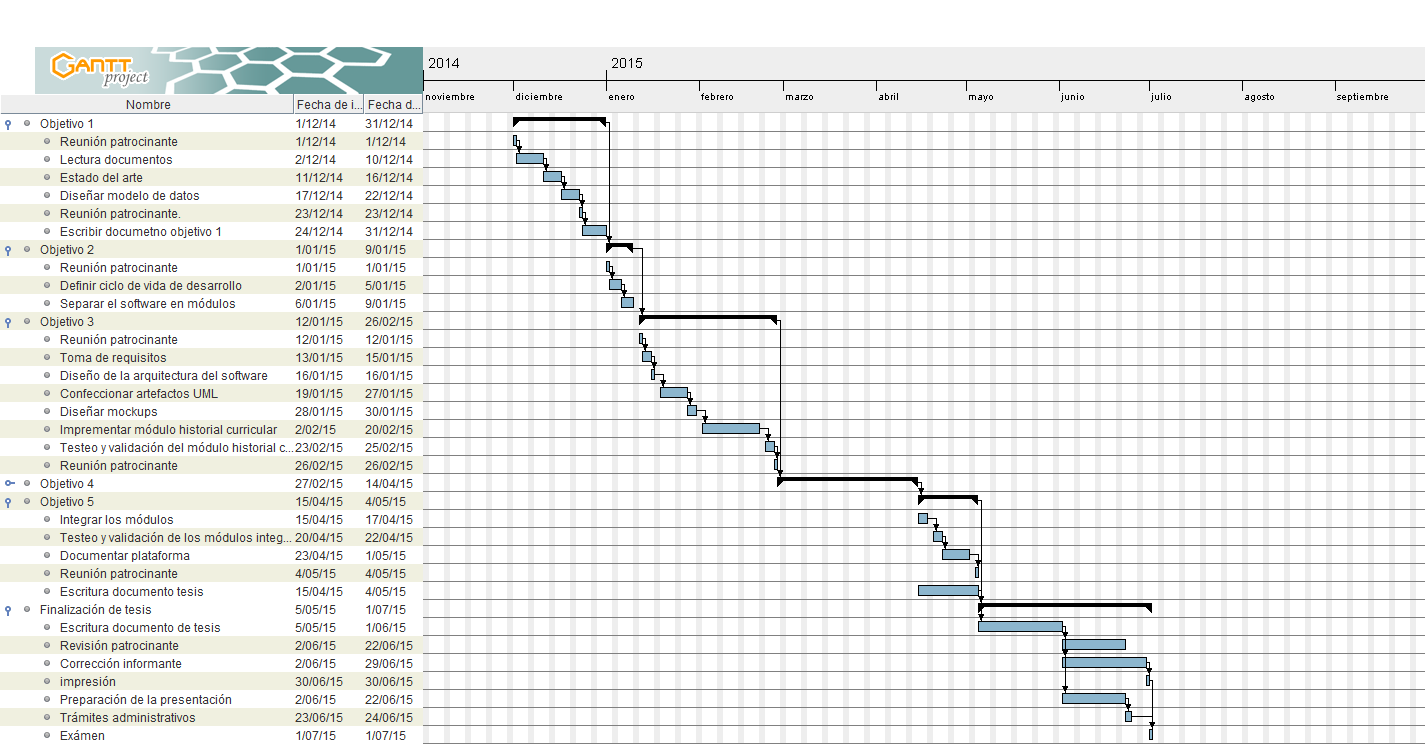
\includegraphics[width=1\textwidth]{images/Capitulo_3/carta_gantt.png}
		\caption[Carta Gantt que exhibe las etapas de desarrollo del sistema]{Carta Gantt que exhibe las etapas de desarrollo del sistema \footnote{}}
		\label{figura_cartaGantt}
	\end{figure}
	\footnotetext{Elaboración propia.}

	Durante el proceso de desarrollo del producto software es importante tener en cuenta lo siguiente:
	\begin{itemize}
		\item Es importante reunirse con el profesor patrocinante al comienzo, durante y al
		término de una iteración, para así aclarar y resolver requerimientos específicos del
		sistema que puedan surgir.
		\item El producto final se dará terminado cuando se hayan cumplido todos los requisitos
		del sistema.
	\end{itemize}

\subsection{Análisis}
	En esta sección se describen los requerimientos y casos de uso más representativos de cada módulo, los cuales fueron obtenidos y discutidos mediante  reuniones con el profesor patrocinador, con el objetivo de identificar los requisitos funcionales y no funcionales que deberían satisfacer el producto software final.
		
	\subsubsection{Requerimientos}
	A continuación se presenta una lista de los requisitos que se definieron para el producto software.

	\myparagraph{Requisitos funcionales}
	
	Los requisitos funcionales del sistema se presentan en la Tabla \ref{Tabla_requisitos_funcionales}.
	\\
	
	
	\begin{longtable}{l |p{11cm}}
	
		\caption{Requisitos funcionales}
		\label{Tabla_requisitos_funcionales}\\

		
		\hline
		\endfirsthead
		\multicolumn{2}{c}%
		{\tablename\ \thetable\ -- \textit{Continuación de la pagina anterior}} \\
		\hline
	
		\hline
		\endhead
		\hline \multicolumn{2}{r}{\textit{Continúa en la página siguiente}} \\
		\endfoot
		\hline
		\endlastfoot
		\rowcolor{LightBlue2} REQF-01 & Autentificación de usuario\\ \hline
		\textbf{Descripción} & El sistema debe ser capaz de diferenciar distintos tipos de usuarios, mediante el RUT, tipo de usuario y contraseña. Estos pueden ser de tres tipo: Administrador, Editor, y Subscriptor.\\ \hline \hline
		
		\rowcolor{LightBlue2} REQF-02 & Gestión de perfil\\ \hline
		\textbf{Descripción} & El sistema debe permitir que los usuarios puedan modificar su contraseña. Además  debe permitir que el Administrador pueda modificar los datos que el usuario ingresó al momento de registrarse.\\ \hline \hline
		
		\rowcolor{LightBlue2} REQF-03 & Desplegar historial curricular\\  \hline
		\textbf{Descripción} &El sistema debe permitir que  todos los usuarios  puedan ver el conjunto de hitos curriculares de una carrera en particular, mediante la facultad, la escuela y la carrera previamente ingresados por el usuario.\\ \\ \\
		\\  \hline \hline
		
		\rowcolor{LightBlue2} REQF-04 & Registro de usuarios\\ \hline
		\textbf{Descripción} & El sistema deberá permitir el registro de nuevos usuarios, los cuales deben ser creados por el Administrador. Los datos a solicitar son: RUT, nombre, apellido paterno, apellido materno, correo electrónico y rol. La contraseña será los 6 primeros dígitos del  RUT ingresado.\\ \hline
		
		\rowcolor{LightBlue2} REQF-05 & Gestión de documentos\\  \hline
		\textbf{Descripción} & El sistema debe permitir al Administrador y Editor crear nuevos registros curriculares, indicando el plan de estudio, la carrera y el tipo de hito: Modificación mayor, Modificación menor o Innovación Curricular, además  debe permitir subir uno o mas archivos en formato PDF por registros, los cuales el sistema los  tienen que clasificar en: Resolución, Comunicación Interna y Petición de requisitos.\\  \hline
		
		\rowcolor{LightBlue2} REQF-07 & Visor de PDF\\  \hline
		\textbf{Descripción} & El sistema debe permitir al usuario ver  cualquier documento que se encuentre almacenado en la base de datos.\\  \hline \hline
		
		
		\rowcolor{LightBlue2} REQF-08 & Notificaciones\\  \hline
		\textbf{Descripción} & El sistema desplegará distintos tipos de notificaciones al momento de realizar cualquier tipo de cambio (guardar, editar, eliminar). Los dos tipos de alertas que se consideraron en la plataforma web son : \textbf{Success} y \textbf{Error}. \\  \hline \hline
		
		\rowcolor{LightBlue2} REQF-09 & Almacenar bitácora de los usuarios\\  \hline
		\textbf{Descripción} & El sistema internamente debe almacenar todas las notificaciones de los eventos ocurridos en la plataforma a fin de tener un registro de  todas  las actividades  que realizan los usuarios en la plataforma. Un registro de la bitácora debe tener necesariamente esta compuesto por: Código de la alerta, mensaje de la alerta, fecha y el RUT de usuario quien ejecutó dicha alerta.\\  \hline
		
		\rowcolor{LightBlue2} REQF-10 & Visualización de bitácora\\  \hline
		\textbf{Descripción} & El sistema debe permitir al administrador visualizar todos los eventos ocurridos en el sistama.\\ 
	
	\end{longtable}

	\myparagraph{Requisitos no funcionales}
	Los requisitos no funcionales se presentan en la Tabla \ref{Tabla_requisitos_no_funcionales}.
	\\

	\begin{longtable}{l |p{11cm}}
		
		\caption{Requisitos no funcionales}
		\label{Tabla_requisitos_no_funcionales}\\
		
		
		\hline
		\endfirsthead
		\multicolumn{2}{c}%
		{\tablename\ \thetable\ -- \textit{Continuación de la pagina anterior}} \\
		\hline
		
		\hline
		\endhead
		\hline \multicolumn{2}{r}{\textit{Continúa en la página siguiente}} \\
		\endfoot
		\hline
		\endlastfoot
	
			\rowcolor{LightBlue2} REQNF-01 & Ambiente Web\\ \hline
			\textbf{Descripción} & El sistema debe visualizarse y funcionar correctamente en cualquier navegador, especialmente en Internet Explorer, Mozilla y Google Chrome.\\ \hline \hline
			
			\rowcolor{LightBlue2} REQNF-02 & Escalabilidad\\ \hline
			\textbf{Descripción} & El sistema debe estar en capacidad de permitir en el futuro el desarrollo de nuevas funcionalidades, modificar o eliminar funcionalidades.\\  \hline
			
			\rowcolor{LightBlue2} REQNF-03 & Facilidad de uso\\ \hline
			\textbf{Descripción} & La interfaz del sistema debe ser amigable con el usuario, Mensajes de errores y éxito.\\ \hline
			
	
			
			\rowcolor{LightBlue2} REQNF-04 & Facilidad de pruebas\\ \hline
			\textbf{Descripción} & El sistema debe contar con facilidad para la identificación de la localización de los errores durante la etapa de prueba.\\ \hline \hline
			
			\rowcolor{LightBlue2} REQNF-05 & Validación\\ \hline
			\textbf{Descripción} & El sistema tiene que poseer una interfaz en la cual se validen los campos obligatorios y  manejo de datos que se ingresan.\\ 
	\end{longtable}

	\subsubsection{Modelo conceptual}
	Para facilitar la compresión de la problemática que se desea solucionar mediante el producto software, en la Figura \ref{Figura_Modelo_conceptual}  se presenta un modelo conceptual, que muestra el dominio dentro del cual se encuentra inmerso el proyecto.
	\\
		\begin{figure}[H]
			\centering
			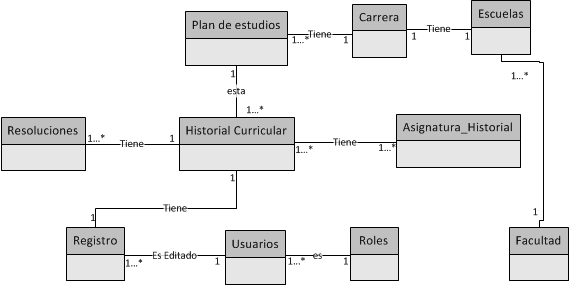
\includegraphics[width=1\textwidth]{images/Capitulo_3/Modelo_Conceptual.png}
			\caption[Modelo conceptual del proyecto]{Modelo conceptual del proyecto \footnote{}}
			\label{Figura_Modelo_conceptual}
		\end{figure}
		\footnotetext{Elaboración propia.}
	\subsubsection{Casos de uso}
	En las Figuras \ref{caso_uso_Administrador}, \ref{caso_uso_Editor}, \ref{caso_uso_Suscriptor} se presentan los diferentes casos de uso para los actores
	involucrados en el sistema.
	
	
	\begin{figure}[H]
		\centering
		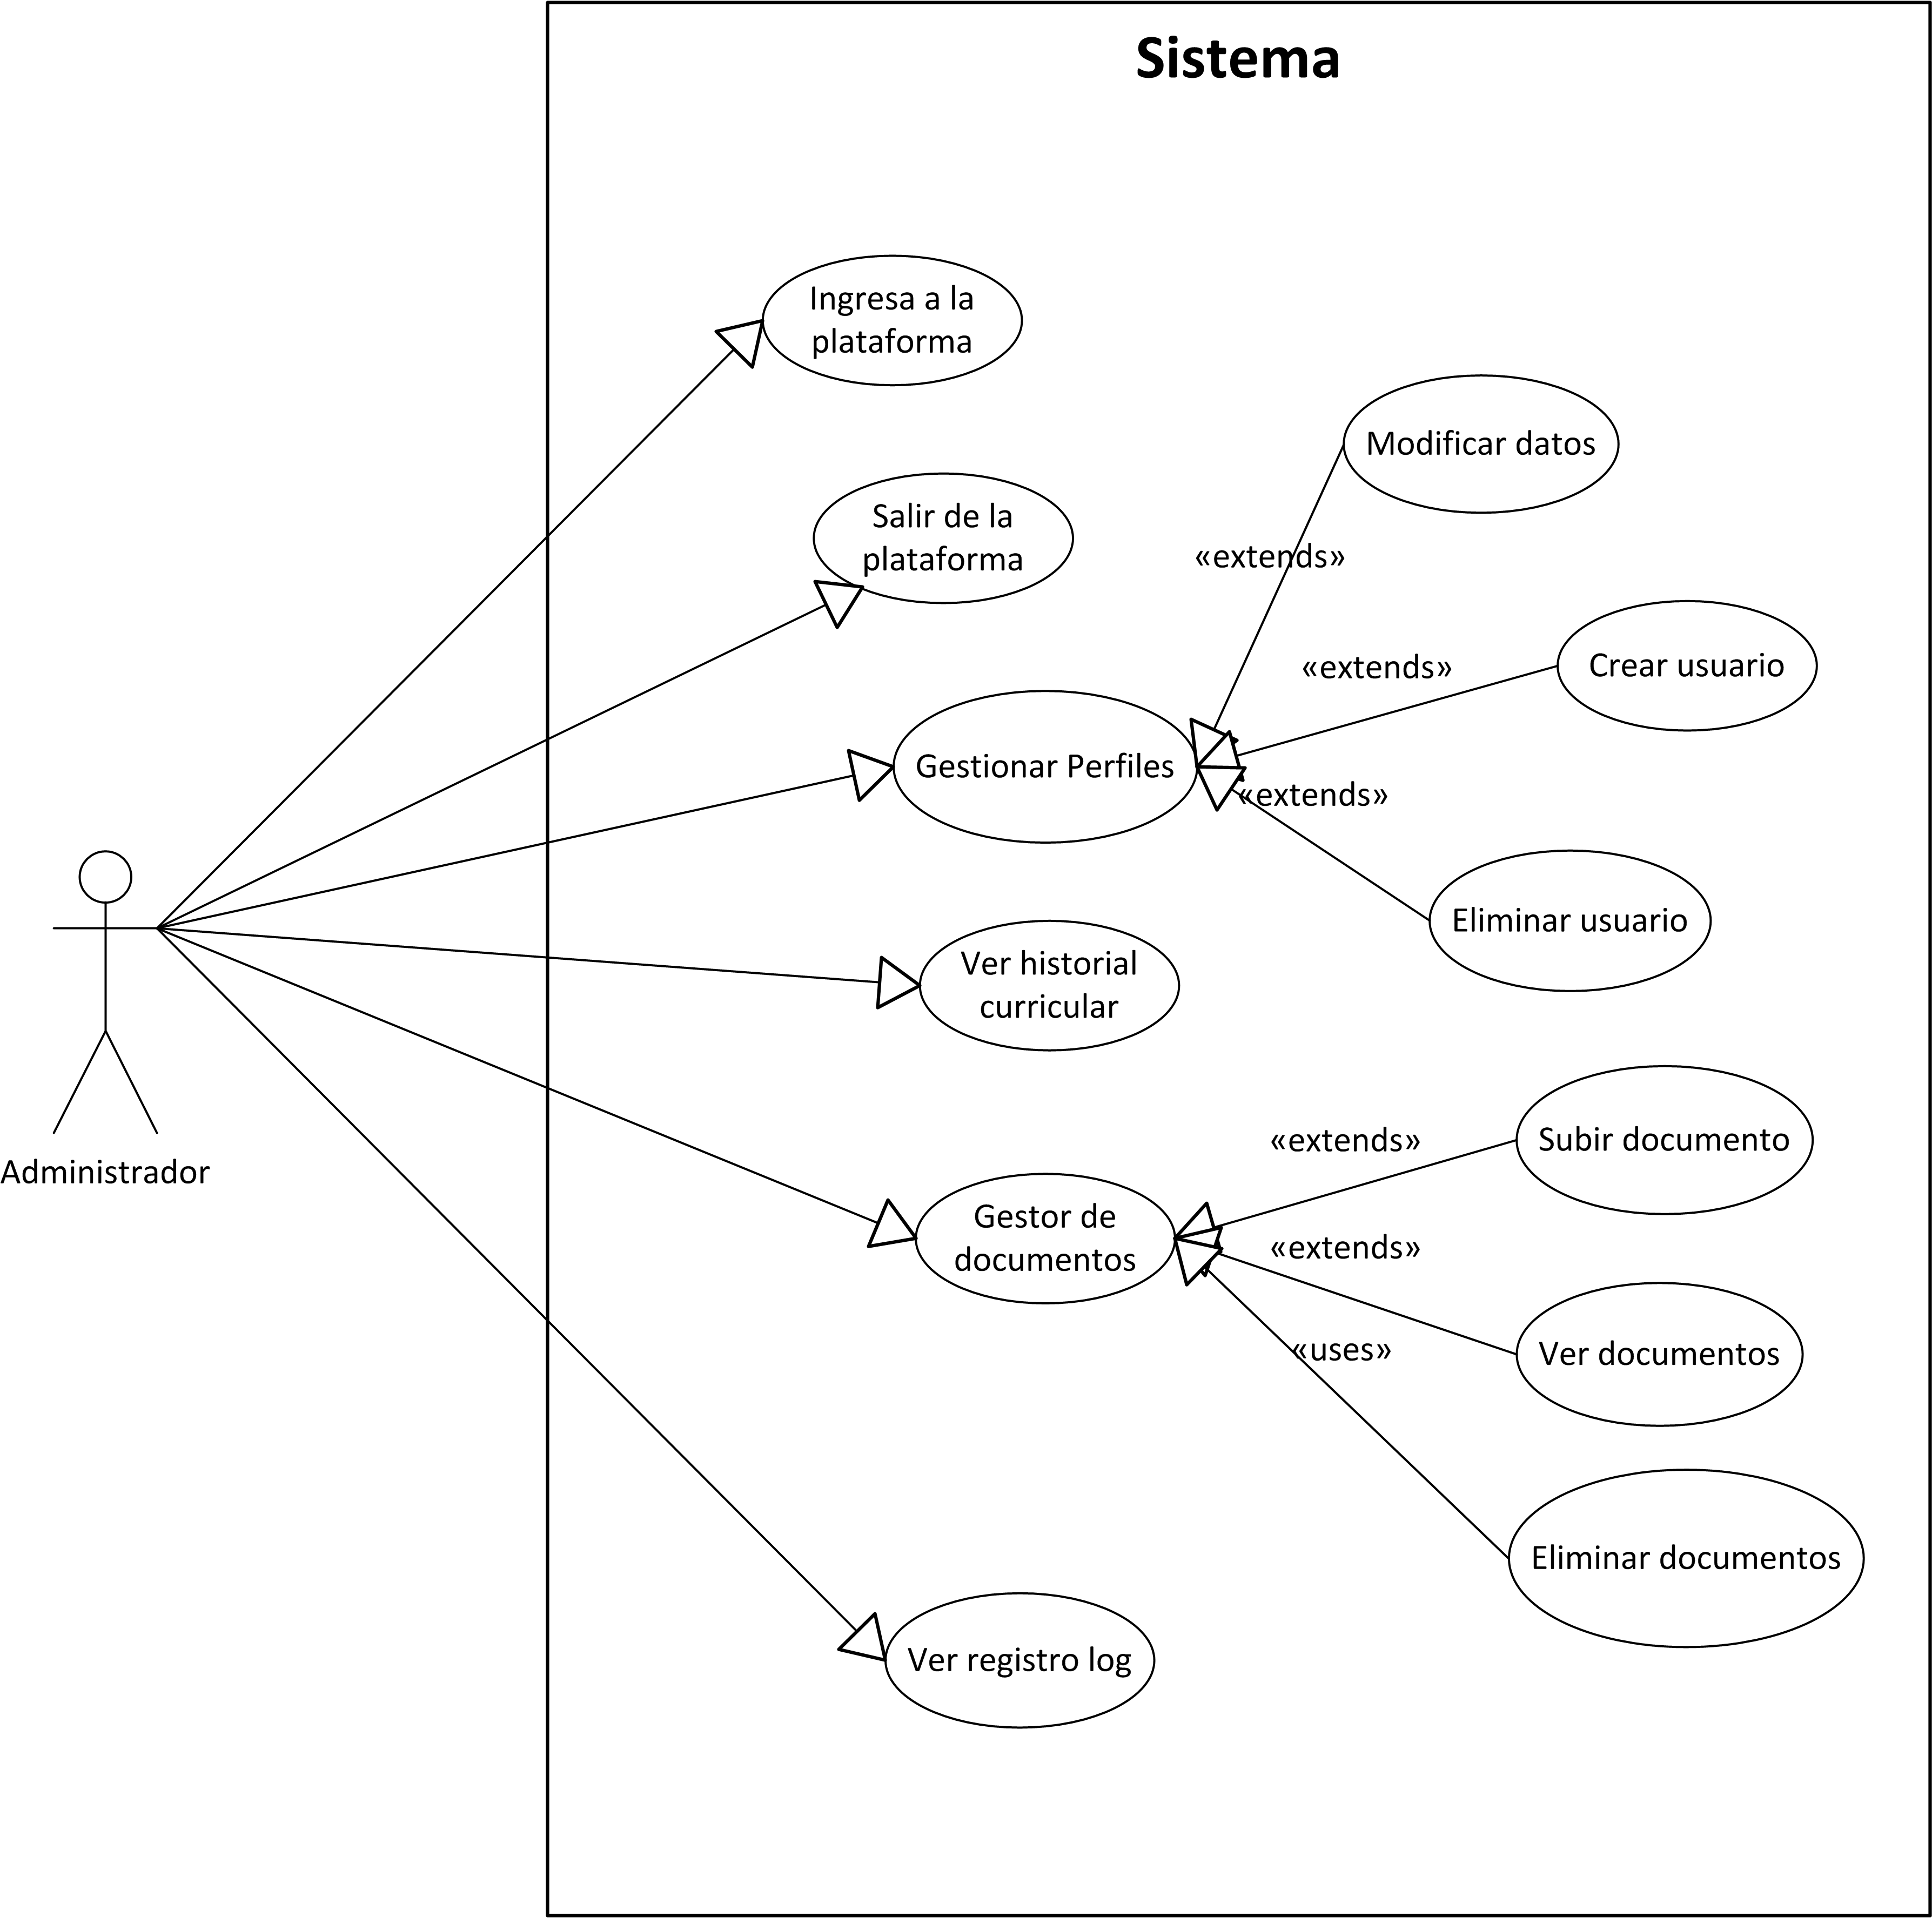
\includegraphics[width=1\textwidth]{images/Capitulo_3/caso_uso_Administrador.png}
		\caption[Diagrama de caso de uso para el Administrador]{Diagrama de caso de uso para el Administrador \footnote{}}
		\label{caso_uso_Administrador}
	\end{figure}
	\footnotetext{Elaboración propia.}
	
	\begin{figure}[H]
		\centering
		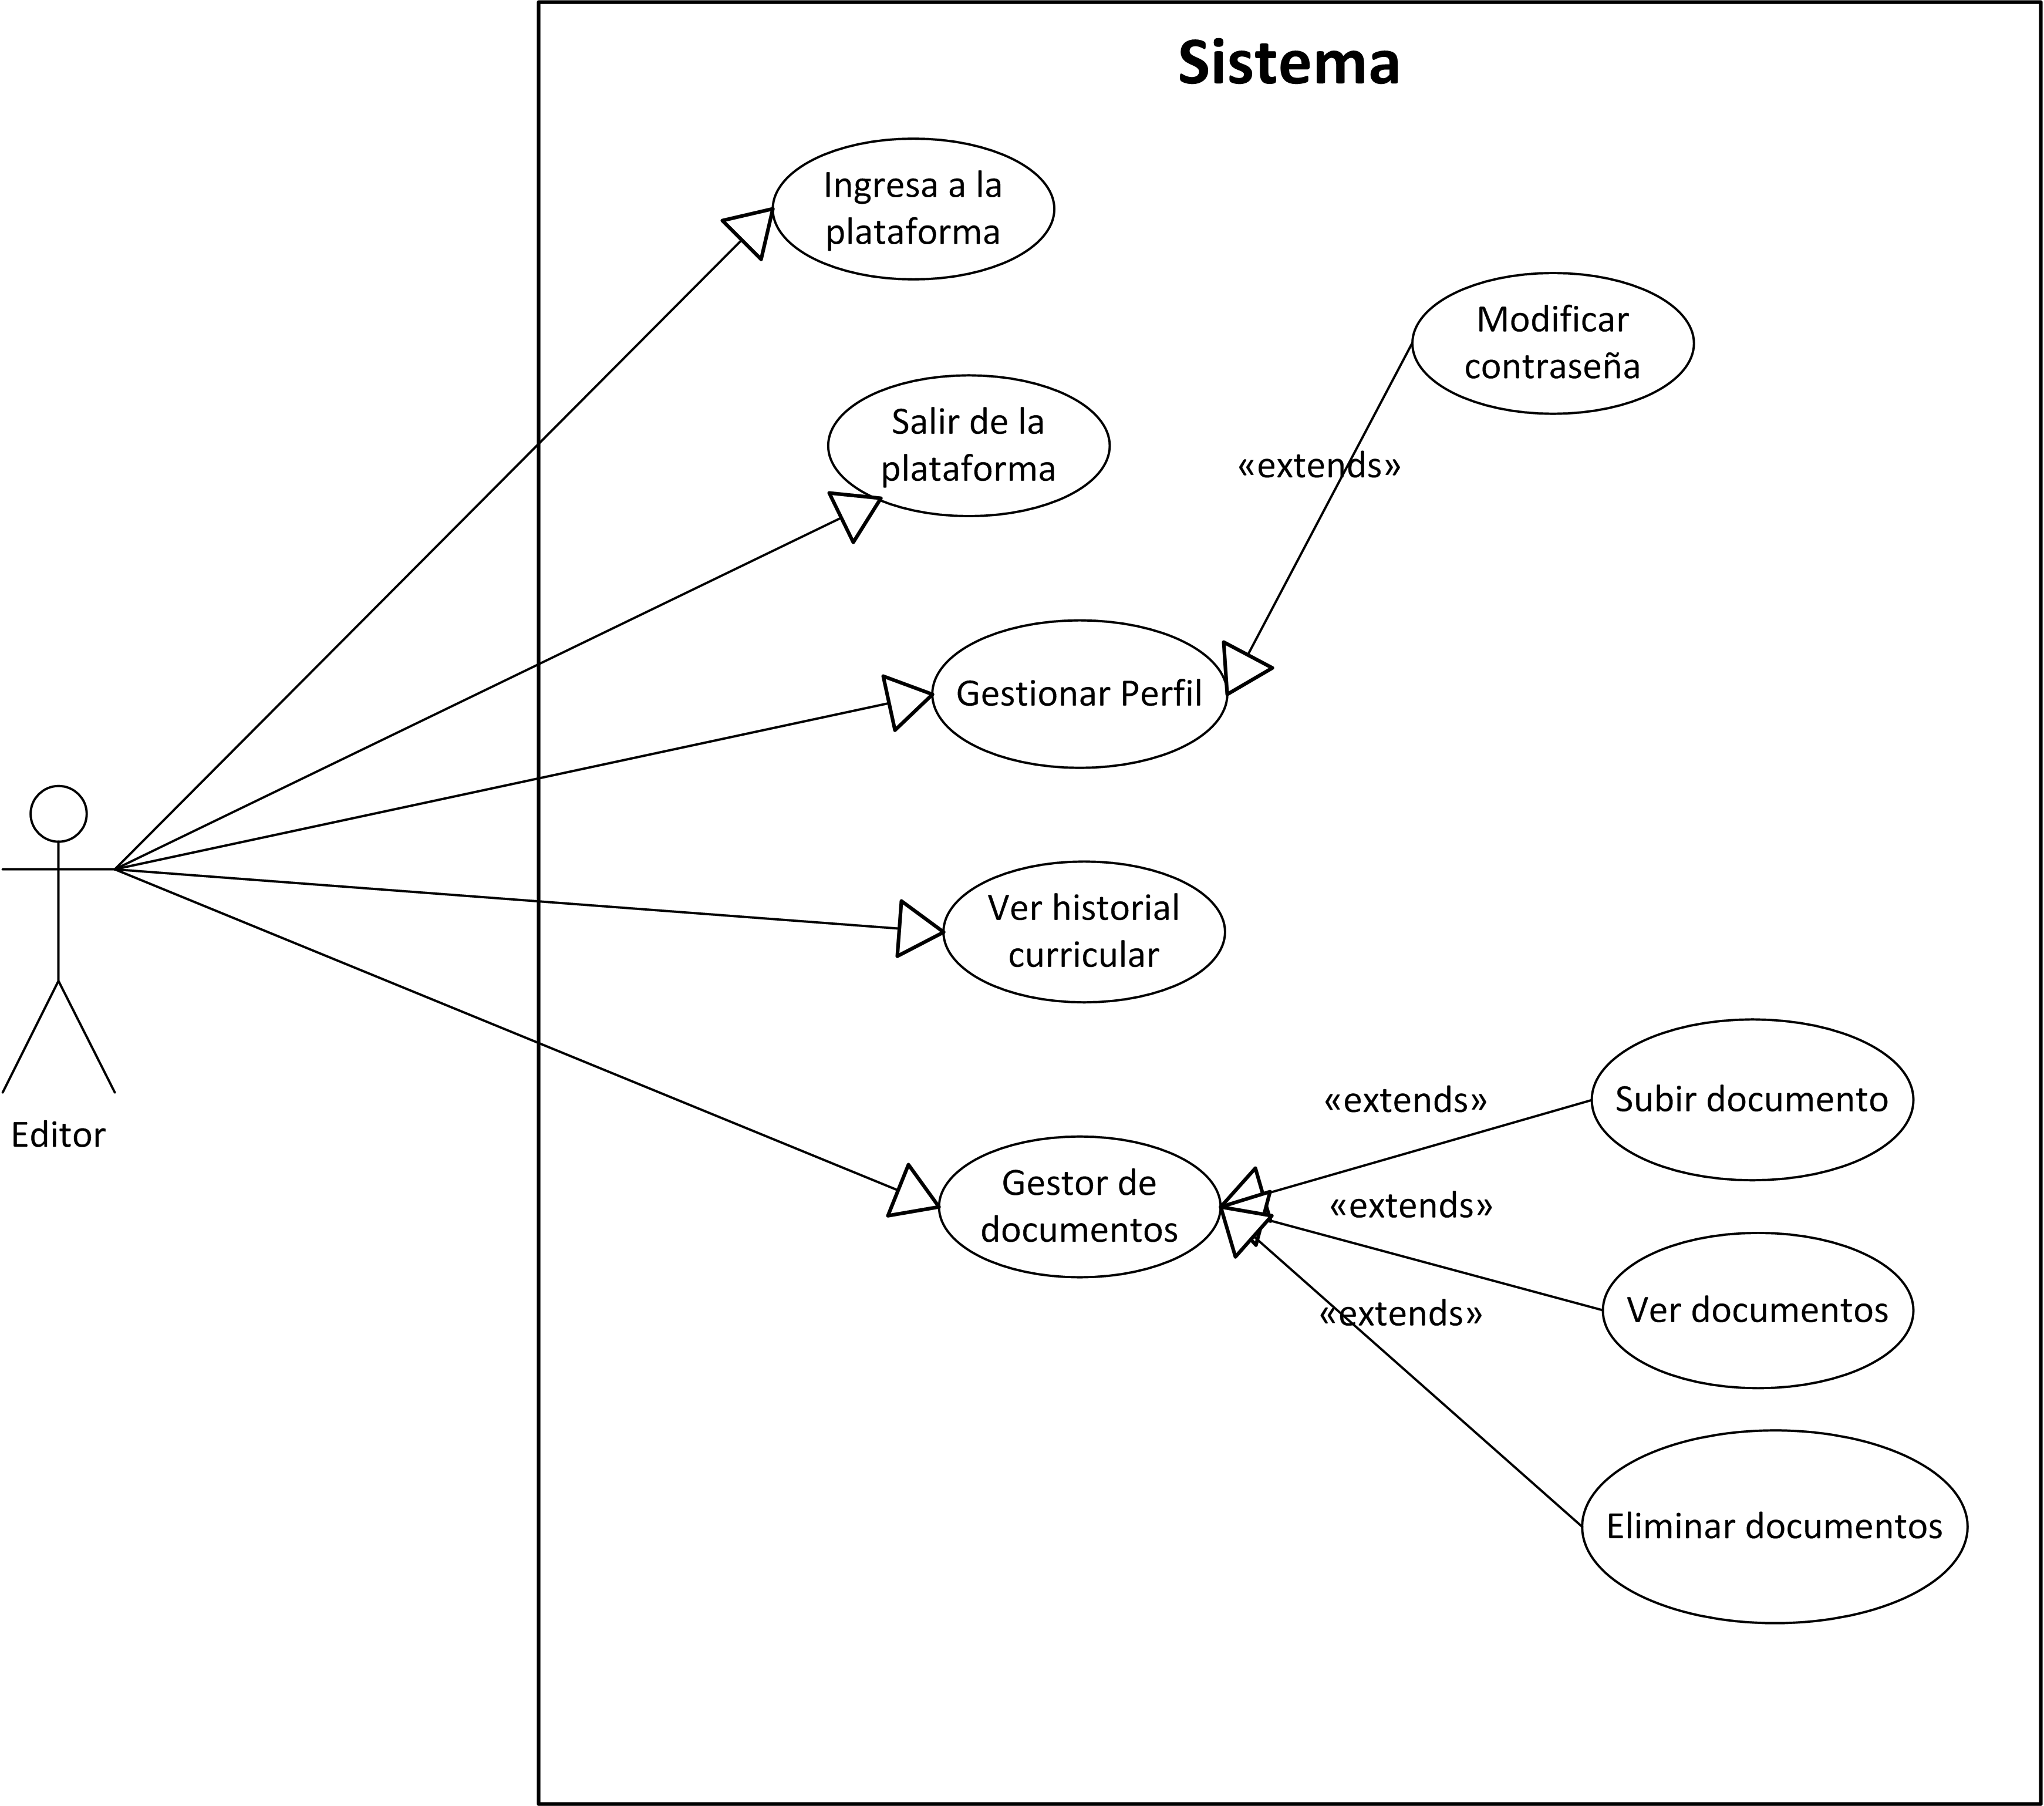
\includegraphics[width=1\textwidth]{images/Capitulo_3/caso_uso_Editor.png}
		\caption[Diagrama de caso de uso para el Editor]{Diagrama de caso de uso para el Editor \footnote{}}
		\label{caso_uso_Editor}
	\end{figure}
	\footnotetext{Elaboración propia.}
	
	\begin{figure}[H]
		\centering
		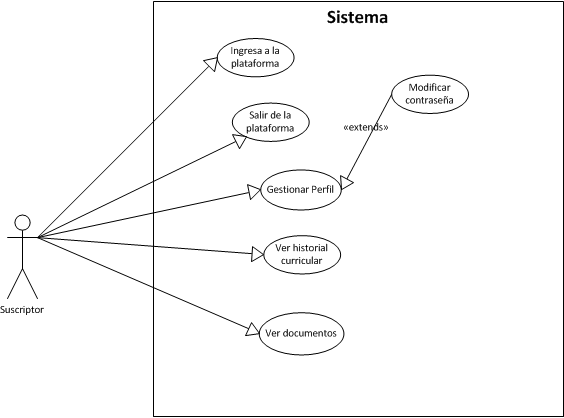
\includegraphics[width=1\textwidth]{images/Capitulo_3/caso_uso_Suscriptor.png}
		\caption[Diagrama de caso de uso para el Suscriptor]{Diagrama de caso de uso para el Suscriptor \footnote{}}
		\label{caso_uso_Suscriptor}
	\end{figure}
	\footnotetext{Elaboración propia.}
	
	\myparagraph{Descripción de los actores del sistema} \label{usuarios_Sistema}
	
	
	\textbf{Suscriptor:} corresponde al grupo de individuos que pueden revisar los datos en la plataforma, es decir, pueden ver el historial curricular de una carrera y ver todas las resoluciones. sin embargo no posee ningún permiso de edición o creación.
	\\
	
	\textbf{Editor:} Este grupo de individuos posee todos los permisos necesarios para poder realizar todas las operaciones básicas (crear, leer,editar y borrar) sobre los registros curriculares y/o los documentos que están en el sistema.
	\\
	
	\textbf{Administrador:} Corresponde al individuo o grupo de individuos que tiene todas las
	funciones de un creador de registros curriculares, pero que además es el encargado de administrar la
	totalidad de usuarios de la plataforma, lo cual incluye el registro, edición y eliminación
	de usuarios.
	
	
	
\subsection{Diseño e implementación}

	En esta sección se describe el diseño y la implementación para los módulos: \textit{Historial curricular} y \textit{Gestor de documentos} de la plataforma. En un principio se muestran algunos artefactos generales correspondientes al diagrama de componentes y al modelo de datos. Posteriormente para cada módulo se presentaran los casos de uso, además del diagrama de secuencia correspondiente.


	\subsubsection{Diagramas de componentes}
	
	En la Figura \ref{diagrama_Componente_SW} y \ref{diagrama_Componente_HW} se muestran los diagramas de componentes software y hardware respectivamente. Ambos diagramas son congruentes con lo visto en el Capítulo \ref{PseudoMVC}, correspondiente al patrón de diseño de programación que utiliza ASP.NET.
			\begin{figure}[H]
				\centering
				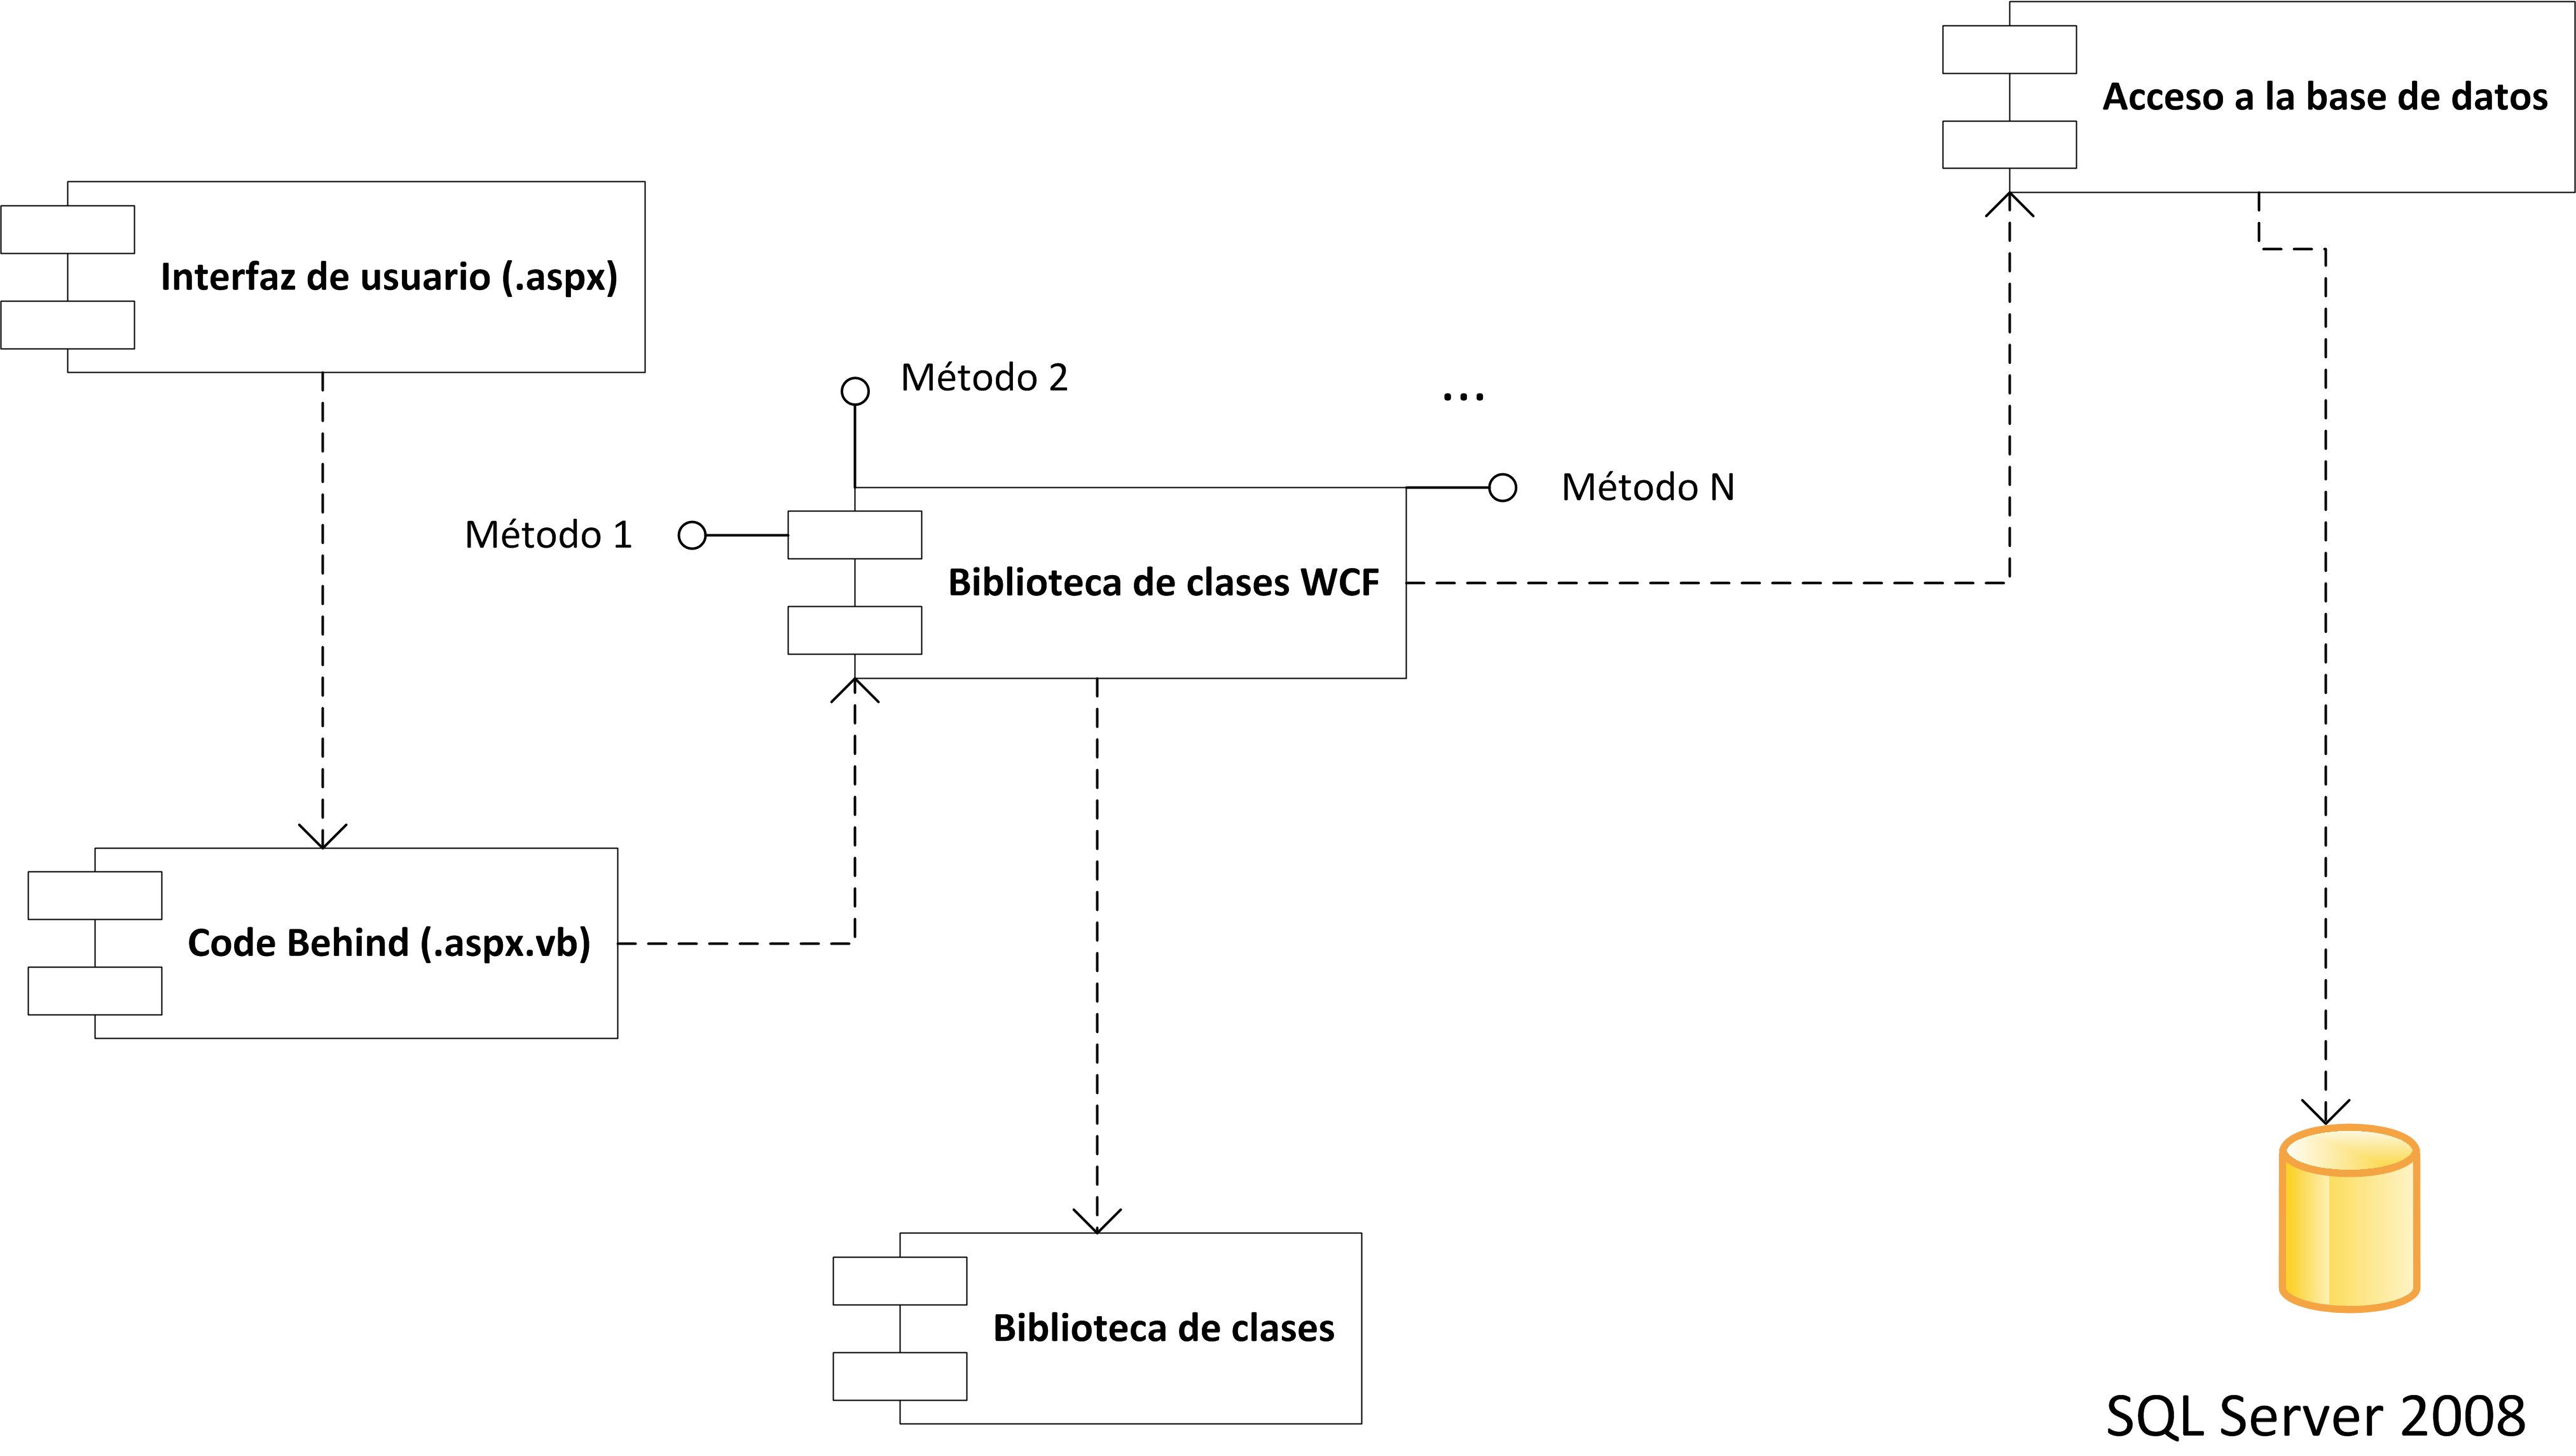
\includegraphics[width=1\textwidth]{images/Capitulo_3/Componente_SW.png}
				\caption[Diagrama de componentes Software del sistema]{Diagrama de componentes Software del sistema\footnote{}}
				\label{diagrama_Componente_SW}
			\end{figure}
			\footnotetext{Elaboración propia.}
	\begin{itemize}
		\item \textbf{Interfaz de usuario:} La interfaz de usuario  consta de los archivos aspx, los cuales no solo definen la estructura de las páginas en el sistema sino también  es el encargado de llamar todos los archivos CSS y JS necesarios para el correcto funcionamiento.
		
		
		\item \textbf{Code Behind:} Como se mencionó en la Sección \ref{ASP.NET}, ASP.NET permite organizar  los eventos  en forma separada de la interfaz. Todo lo relacionado con Interfaz de usuario se maneja en el archivo .aspx y el control de los eventos en un archivo separado .aspx.vb.
		
		\item \textbf{biblioteca de clases WCF:} Este componente contiene los servicios web de la aplicación.
		
		\item \textbf{biblioteca de clases:} Conjunto de clases que definen las estructuras de las  entidades de la base de datos.
		
		\item \textbf{Acceso a la base de datos:} El acceso a la base de datos se realiza  mediante un DLL que fue facilitado por la DTI.
	\end{itemize}		
			
		\begin{figure}[H]
			\centering
			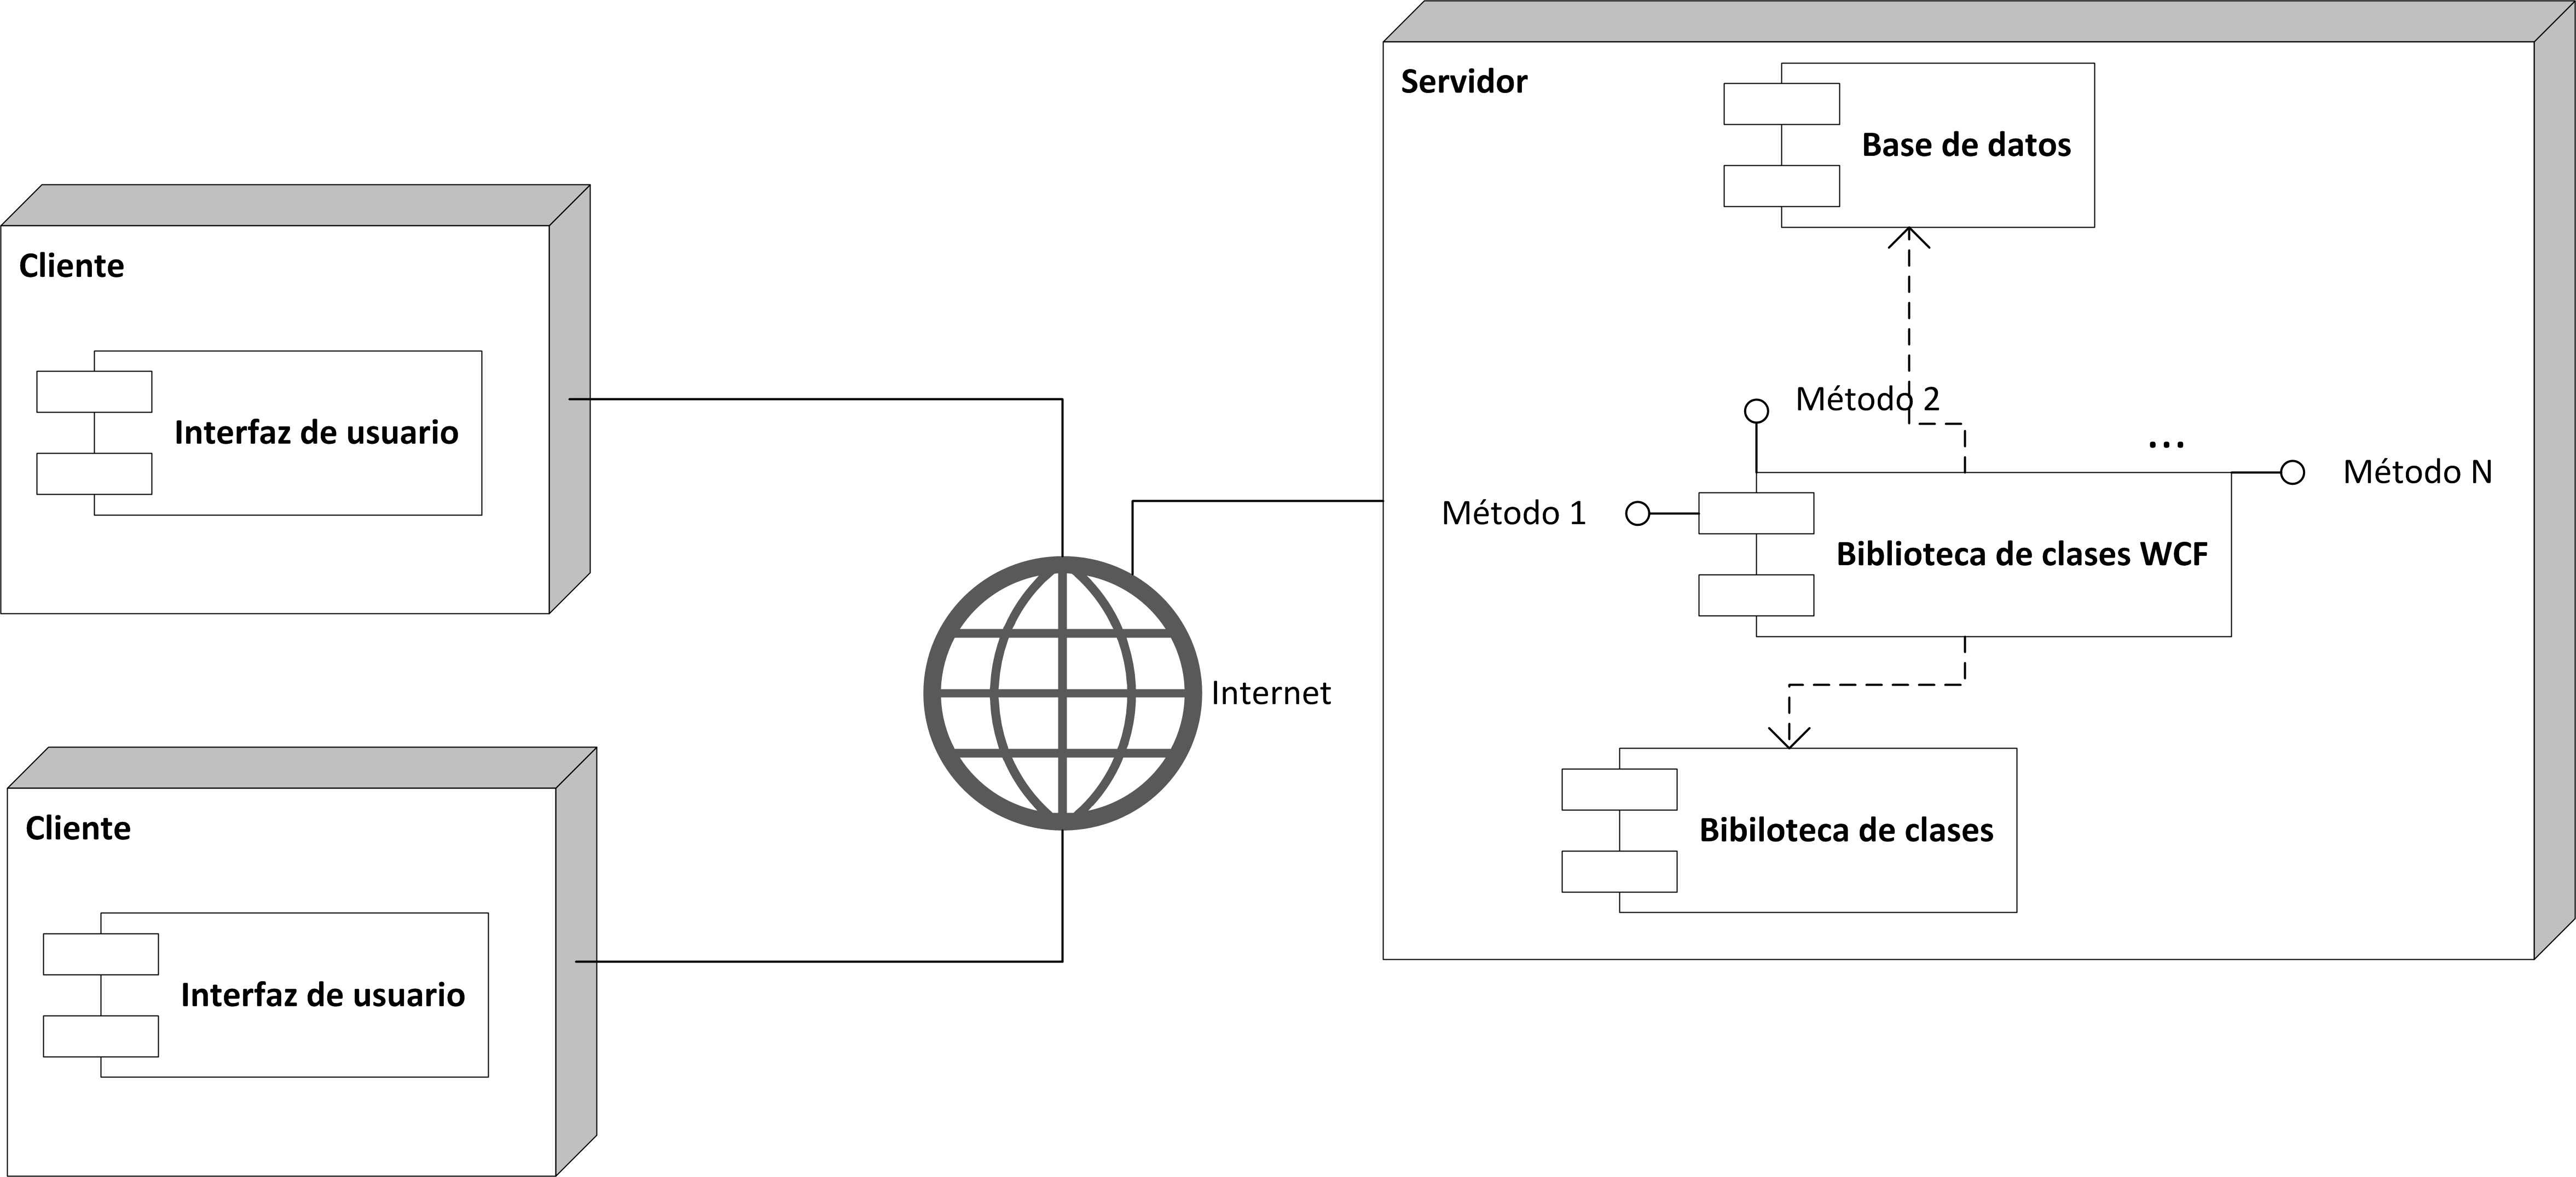
\includegraphics[width=1\textwidth]{images/Capitulo_3/Componente_HW.png}
			\caption[Diagrama de componentes Hardware del sistema]{Diagrama de componentes Hardware del sistema\footnote{}}
			\label{diagrama_Componente_HW}
		\end{figure}
		\footnotetext{Elaboración propia.}
		
	\subsubsection{Modelo de datos}
	
	El contexto en el que se desenvuelve el software contempla 14 entidades, de las cuales 8 de ellas se exportaron desde la base de datos de la Universidad para poder trabajar en un ambiente de desarrollo, estas entidades son: Facultad, Escuelas, Carreras, PlanEstudio, PlanAsignatura, Plan\_asig\_requisito,institutos y asignaturas.
	\\
	
	Las entidades restantes fueron creadas con el fin de satisfacer las necesidades de la problemática en la cual se encuentra inmerso en proyecto. El modelo de datos completo se puede ver en la Figura \ref{Modelo_E_R}.
	\\
	
	\begin{figure}[H]
		\centering
		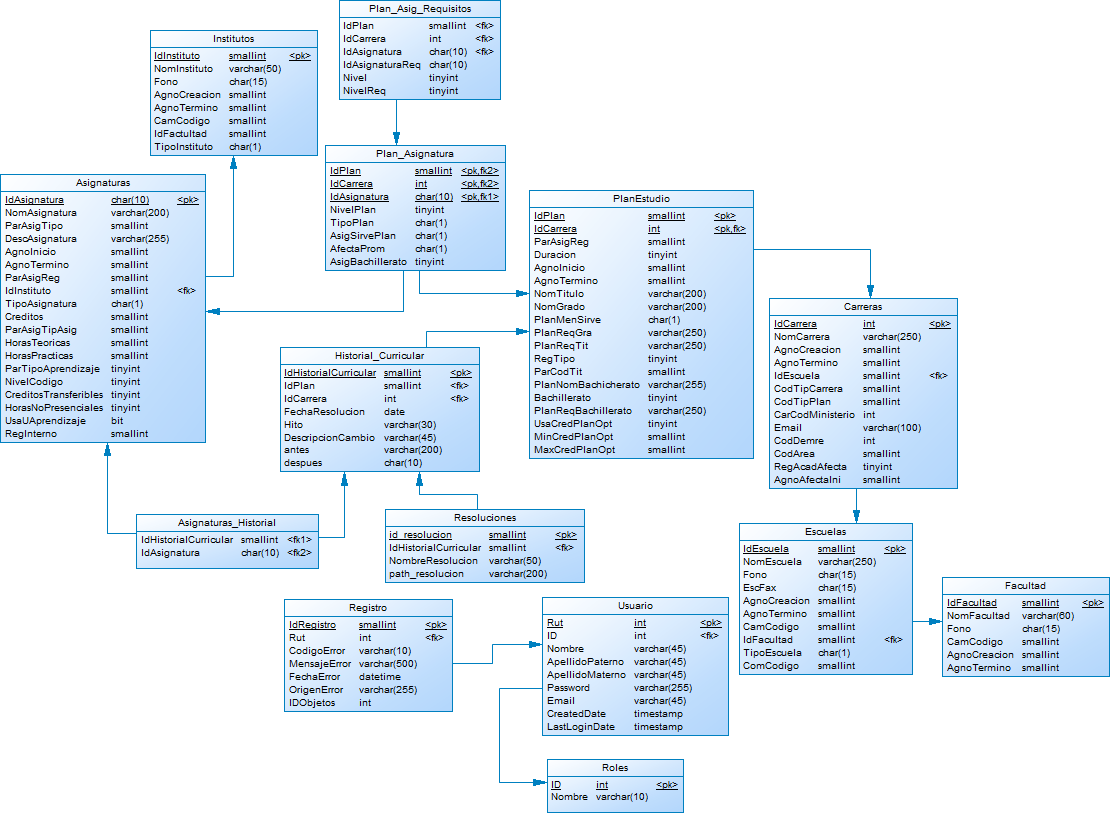
\includegraphics[width=1\textwidth]{images/Capitulo_3/Modelo_E_R.png}
		\caption[Modelo de datos Entidad-Relación]{Modelo de datos Entidad-Relación \footnote{}}
		\label{Modelo_E_R}
	\end{figure}
	\footnotetext{Elaboración propia.}
	
	\myparagraph{Diccionario de datos}
	
	Es importante que todo proyecto el cual involucre un almacenamiento de datos, posea un diccionario de datos, puesto que el  objetivo de un diccionario de datos  es dar precisión sobre los datos	que se manejan en un sistema, evitando así  malas interpretaciones.
	\\
	
	Como se mencionó anteriormente, no todas las entidades son de creación propia, por lo que el en Anexo C se puede ver el diccionario de datos correspondiente solo a las tablas creadas.
	
	
	
	\subsubsection{Módulo historial curricular}
	
	El módulo historial curricular esta diseñado para que todos los usuarios definidos en la Sección \ref{usuarios_Sistema} tengan acceso a él, a causa de que su principal objetivo es ver la trazabilidad de una carrera en particular.
	\myparagraph{Diseño}
	A continuación se describe el diseño del caso de uso más significativo para el módulo  historial curricular de la plataforma, que corresponde a la visualización de la trazabilidad de los planes de estudio de las carreras . Se presentará en detalle la composición de este caso de uso y su participación en el sistema.
		
	\mysubparagraph{ Caso de uso real más significativo} 
	
	El caso de uso “Ver historial curricular” ocurre cuando un usuario  desea  ver los cambios  curriculares que se le han aplicado a una carrera en particular. El caso de uso real “Ver historial curricular” se presenta en la Tabla \ref{Tabla_Caso_Uso_ver_historial}.
	
	
		\begin{longtable}{p{7cm}| p{7cm}}
			
			\caption{Caso de uso Ver historial curricular}
			\label{Tabla_Caso_Uso_ver_historial}\\
			
			
			\hline
			\endfirsthead
			\multicolumn{2}{c}%
			{\tablename\ \thetable\ -- \textit{Continuación de la página anterior}} \\
			\hline
			
			\hline
			\endhead
			\hline \multicolumn{2}{r}{\textit{Continúa en la página siguiente}} \\
			\endfoot
			\hline \hline
			\endlastfoot
			\rowcolor{LightBlue2}  \multicolumn{2}{c}{Caso de Uso Ver Historial Curricular} \\  \hline
			
			
			\textbf{Actores} & Administrador, Editor, Suscriptor.\\ \hline
			
			\textbf{Propósito} & Visualizar los cambios curriculares que se han realizado en una determinada carrera.\\ \hline
			
			\textbf{Tipo} & Primario y esencial\\ \hline
			
			\multicolumn{2}{p{15cm}}{\textbf{Resumen:} Un usuario autentificado puede ver el historial curricular de una carrera en particular, el cual lo hace primero seleccionado la facultad a la que pertenece, luego la escuela y por último selecciona la carrera en cuestión.} \\  \hline \hline
			 
			\rowcolor{LightBlue2}  \multicolumn{2}{c}{Interfaz: Formulario Ver Historial Curricular} \\  \hline \hline
			
			\multicolumn{2}{c}{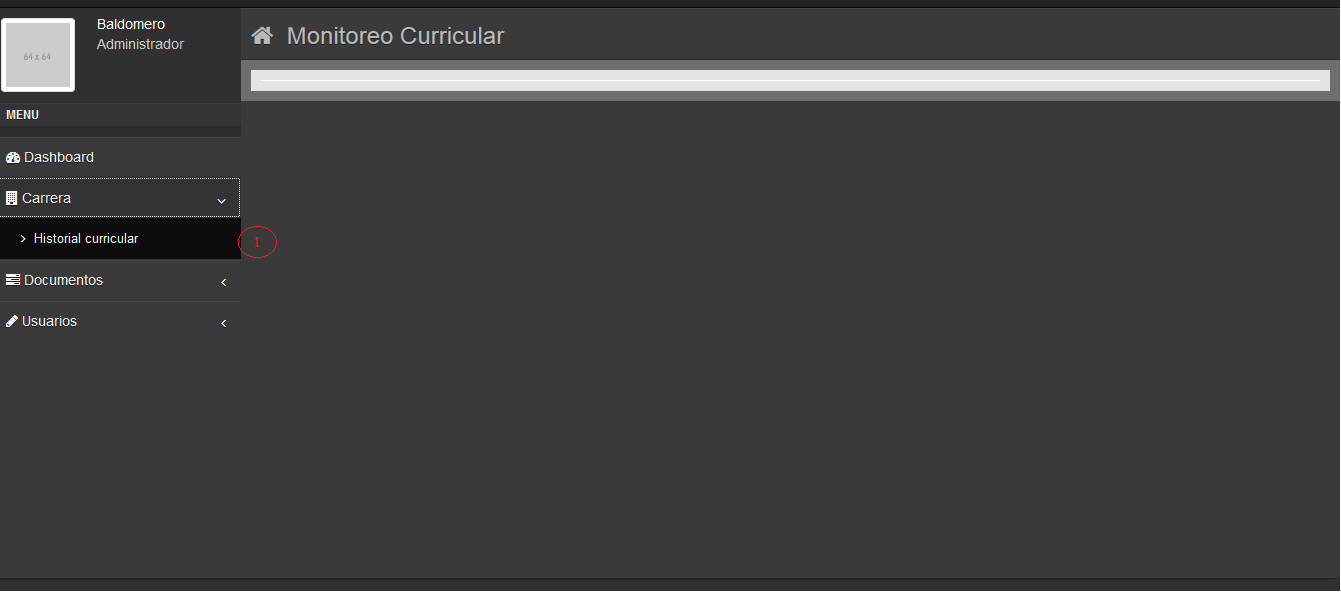
\includegraphics[width=1\textwidth]{images/Capitulo_3/F_historialCurricular1.png}} \\ 
			
			\multicolumn{2}{c}{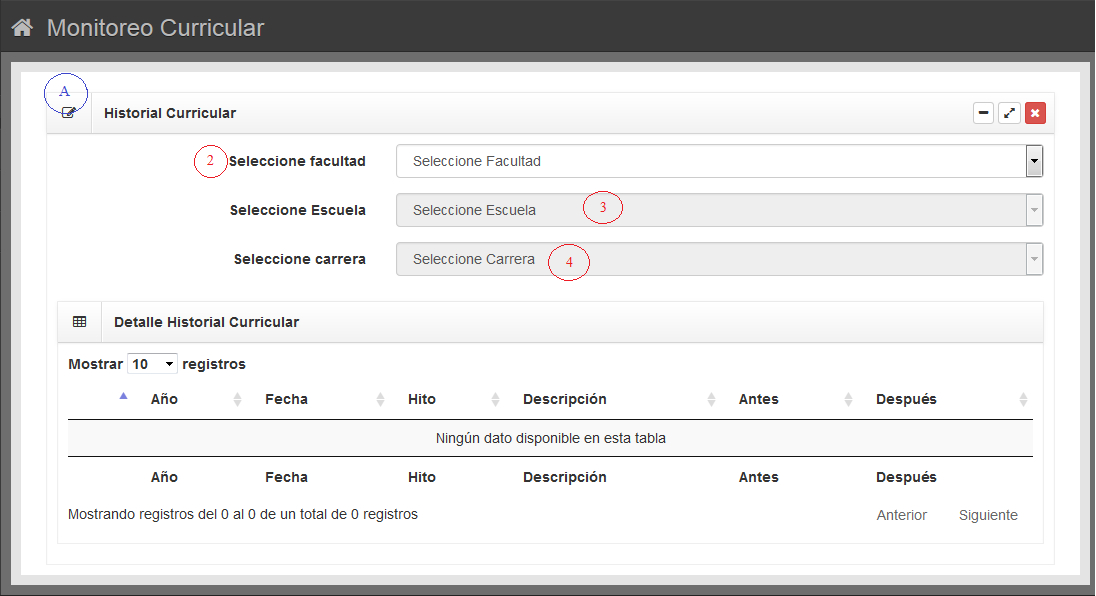
\includegraphics[width=1\textwidth]{images/Capitulo_3/F_historialCurricular2.png}} \\ 
			
			\multicolumn{2}{c}{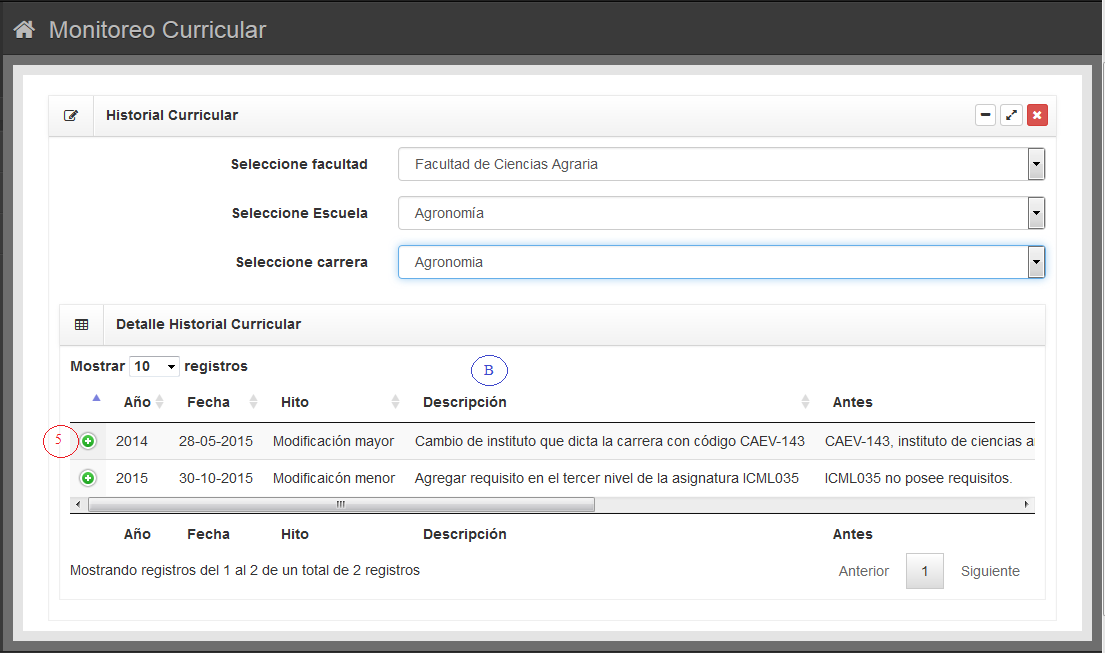
\includegraphics[width=1\textwidth]{images/Capitulo_3/F_historialCurricular3.png}} \\ 
			
			\multicolumn{2}{c}{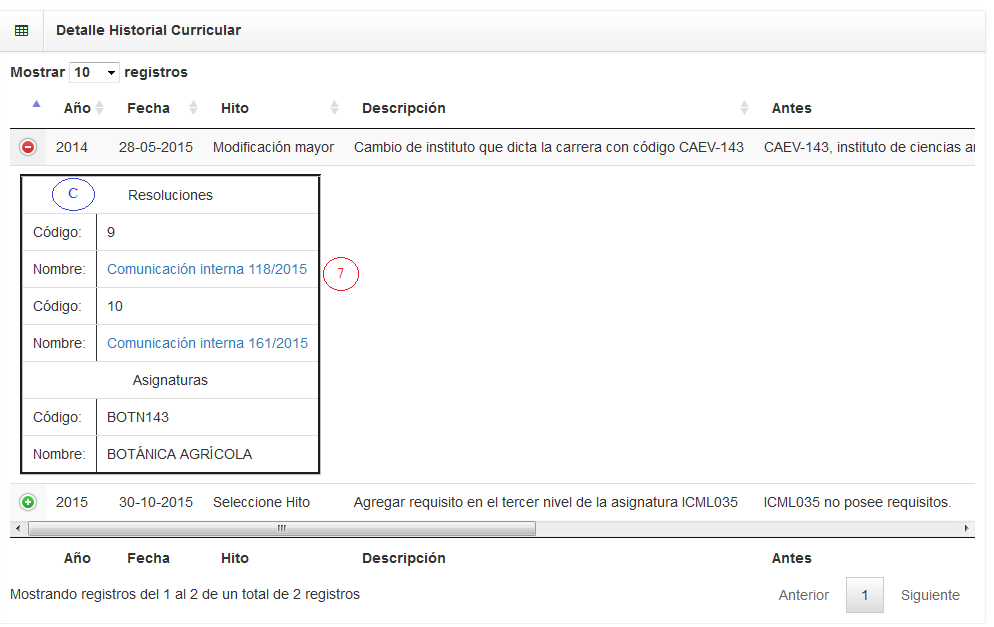
\includegraphics[width=1\textwidth]{images/Capitulo_3/F_historialCurricular4.png}} \\ \hline
			
			\rowcolor{LightBlue2}  \multicolumn{2}{c}{Curso normal de eventos} \\ 
			
			\textbf{Acción actor} &	\textbf{Respuesta sistema} \\ \hline
			
			1.- Este caso de uso comienza cuando un usuario autentificado desea ver el historial curricular de una carrera, para ello debe hacer click en \textbf{1}.
			 &	2.- El sistema despliega la pantalla \textbf{A}, el cual permite al usuario seleccionar facultad, escuela y carrera. \\ \hline
		
		
			3.- El usuario selecciona la facultad, escuela y carrera, haciendo click en \textbf{2},\textbf{3} y \textbf{4}.
			&	4.- El sistema crear un texto plano en formato JSON, el cual contiene el detalle solicitado por el usuario.\\ \hline
			
			
			& 5.- El sistema lee el archivo JSON y lo despliega en la tabla \textbf{B}.\\ \hline
			
			6.- Para ver información mas detallada del hito, el usuario puede hacer click en \textbf{6}.
			&	7.- El sistema despliega la información solicitada en \textbf{C}.\\ \hline
		
		
			8.- Si el usuario lo desea, puede ver la resolución haciendo click en \textbf{7}.
			&	9.- El sistema redirecciona al usuario al documento solicitado.\\ \hline
		\end{longtable}
		
		
		En la Figura \ref{diagrama_secuencial_ver_historial} se presenta el diagrama de secuencia para este mismo caso de uso, y así mostrar la interacción entre los distintos componentes del software que llevan a cabo esta tarea.
		
			\begin{figure}[H]
				\centering
				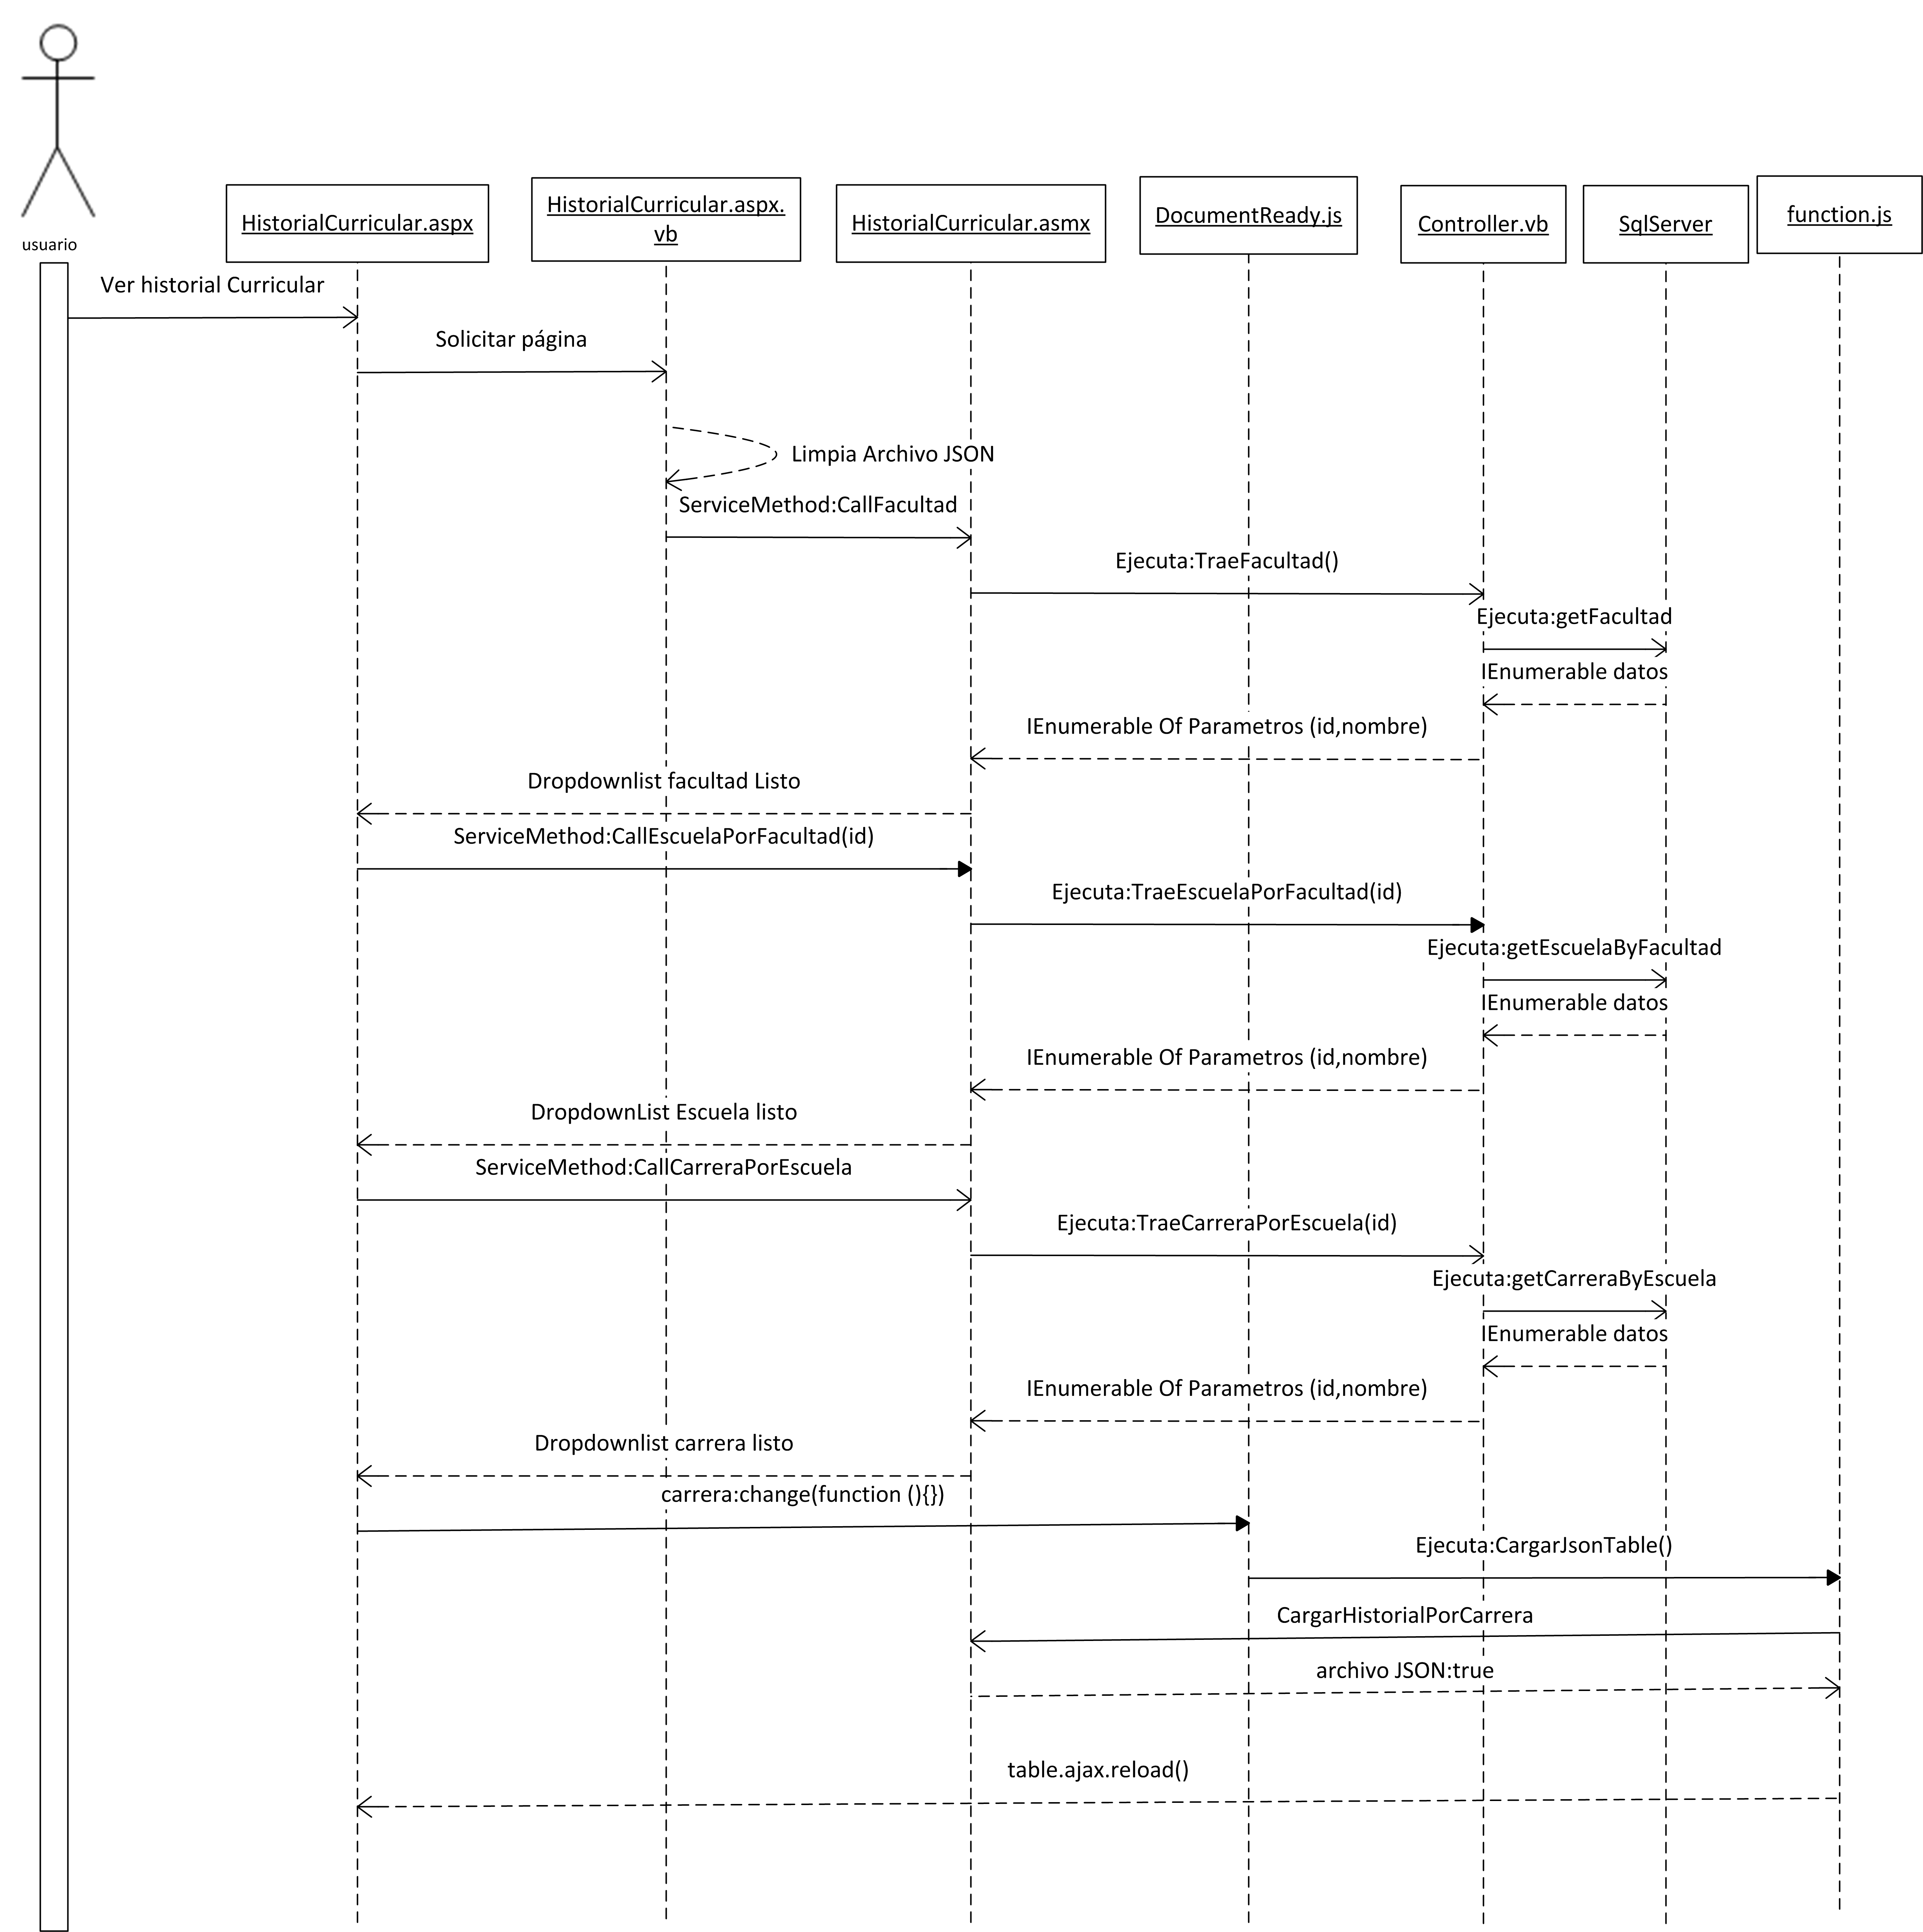
\includegraphics[width=1\textwidth]{images/Capitulo_3/diagrama_secuencial_Historial_Curricular.png}
				\caption[Diagrama de secuencia para el caso de uso \textit{Ver Historial Curricular}]{Diagrama de secuencia para el caso de uso \textit{Ver Historial Curricular} \footnote{}}
				\label{diagrama_secuencial_ver_historial}
			\end{figure}
			\footnotetext{Elaboración propia.}

		
		 En primer lugar el \textit{HistorialCurricular.aspx}  debe asegurarse que el archivo JSON de donde se leen los datos este vacío y con el formato adecuado para su correcta lectura(el formato del arhivo JSON utilizado se puede ver en el Anexo A). Una vez realizada esta acción, la vista se comunica con el servicio web (HistorialCurricular.asmx) para que la primera lista desplegable, correspondiente a las facultades  de la universidad,  no este vacía.\\
		 
		  El proceso que se describirá a continuación es la secuencia de pasos que realiza el sistema para  ``poblar'' una lista desplegable, por lo que este proceso se repite tres veces, la única diferencia es quién activa el proceso. Para la lista desplegable que se llena con las facultades la activa el sistema antes de mostrar el formulario al usuario, mientras que para las listas desplegables que abarcan a las escuelas y a las carreras las activa el usuario al momento de producir un cambio en las listas desplegables de niveles superiores, es decir, 
		  para que  el sistema poble la lista desplegable que contiene a las escuelas, el usuario debe producir un cambio en el DropDownList que contiene a  las facultades, y para poblar el DropDownList que contiene a las carreras, el usuario debe producir un cambio en la lista desplegable que abarca a las escuelas.\\

		
		
	
		El   \textbf{poblado de una lista desplegable} comienza cuando el HistorialCurricular.asmx  envía un mensaje a  la  \label{Proceso_poblado_DDL} biblioteca Controller.vb indicando qué datos se necesitan de la base de datos (Facultad, Escuela o Carrera), una vez que el Controller.vb recibe la petición, ejecuta  la consulta correspondiente y  retorna los datos solicitados en formato IEnumerable al servicio web, con el fin de que éste último actor asigne la información retornada en la lista desplegable correspondiente.
		\\
		
	
		Una vez que  el sistema haya verificado el estado del archivo JSON y que haya poblado la lista desplegable de las facultades, la plataforma esta en condiciones de mostrar el formulario al usuario para su posterior manipulación.		Por otra parte el DocumentReady.js esta a la espera de que el usuario seleccione la carrera, a fin de enviar un mensaje al Function.js con el ID de la carrera.
		\\
		
		Una vez que el actor Function.js reciba el ID de la carrera,  lo envía al servicio web para que éste cree el archivo JSON, tan pronto como se cree el archivo el HistorialCurricular.asmx  envía la variable JSON=true al actor Function.js para que se visualicen los datos del archivo JSON en la interfaz web.
		
		\subsubsection{Módulo Gestor de Documentos}
	
	
		El  módulo Gestor de documentos permite al administrador y editor administrar el repositorio de documentos de la plataforma, dicho de otra manera, estos usuarios podrán: crear, leer, editar y eliminar registros. Con respecto al usuario de tipo suscriptor, solo poseerá permisos de lectura.
	
		\myparagraph{Diseño}
		
		A continuación se describe el diseño de los dos  casos de usos extendidos del módulo de gestión de documentos de la plataforma, que corresponden a: subir documentos y  ver documentos. Se presentará en detalle la composición de estos casos de uso y su participación en el sistema.
		
		\mysubparagraph{ Caso de uso real del módulo gestor de documentos:``Subir documento''} 
		




		El caso de uso ``Subir documento'' corresponde al caso de uso extendido de ``Gestor de documentos'' y  ocurre cuando un administrador o un editor desea crear algún hito curricular en un plan de estudios. El caso de uso real ``Subir documento'' se presenta en la Tabla \ref{Tabla_Caso_Uso_Subir_Documento}.
		
		
		
		
			\begin{longtable}{p{7cm}| p{7cm}}
				
				\caption{Caso de uso  Subir Documento}
				\label{Tabla_Caso_Uso_Subir_Documento}\\
				
				
				\hline
				\endfirsthead
				\multicolumn{2}{c}%
				{\tablename\ \thetable\ -- \textit{Continuación de la página anterior}} \\
				\hline
				
				\hline
				\endhead
				\hline \multicolumn{2}{r}{\textit{Continúa en la página siguiente}} \\
				\endfoot
				\hline \hline
				\endlastfoot
				\rowcolor{LightBlue2}  \multicolumn{2}{c}{Caso de uso  Subir Documento} \\  \hline
				
				
				\textbf{Actores} & Administrador y Editor.\\ \hline
				
				\textbf{Propósito} & Crear un hito curricular a un plan de estudios.\\ \hline
				
				\textbf{Tipo} & Primario y esencial\\ \hline
				
				\multicolumn{2}{p{15cm}}{\textbf{Resumen:} El objetivo de este módulo es hacer posible la creación de hitos curriculares y la carga de documentos relacionados con el hito en cuestión al servidor.} \\  \hline \hline
				
				\rowcolor{LightBlue2}  \multicolumn{2}{c}{Interfaz: Formulario Ver Historial Curricular} \\  \hline \hline
				
				\multicolumn{2}{c}{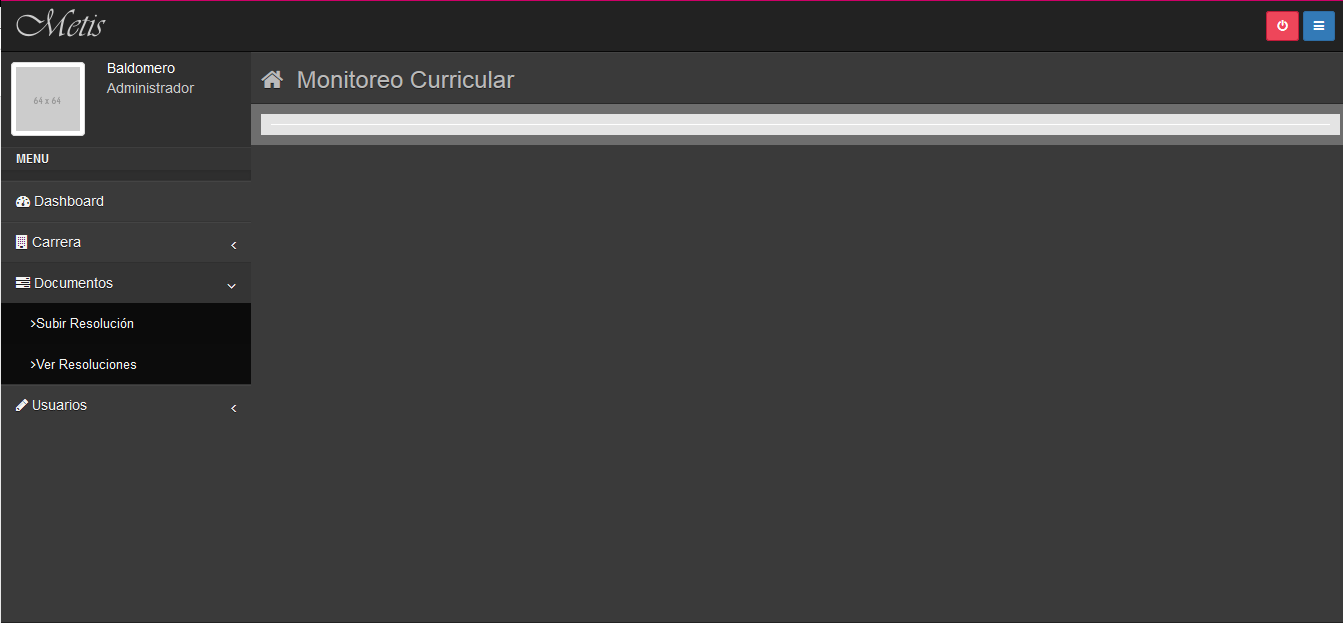
\includegraphics[width=1\textwidth]{images/Capitulo_3/subir_documento1.png}} \\ 
				
				\multicolumn{2}{c}{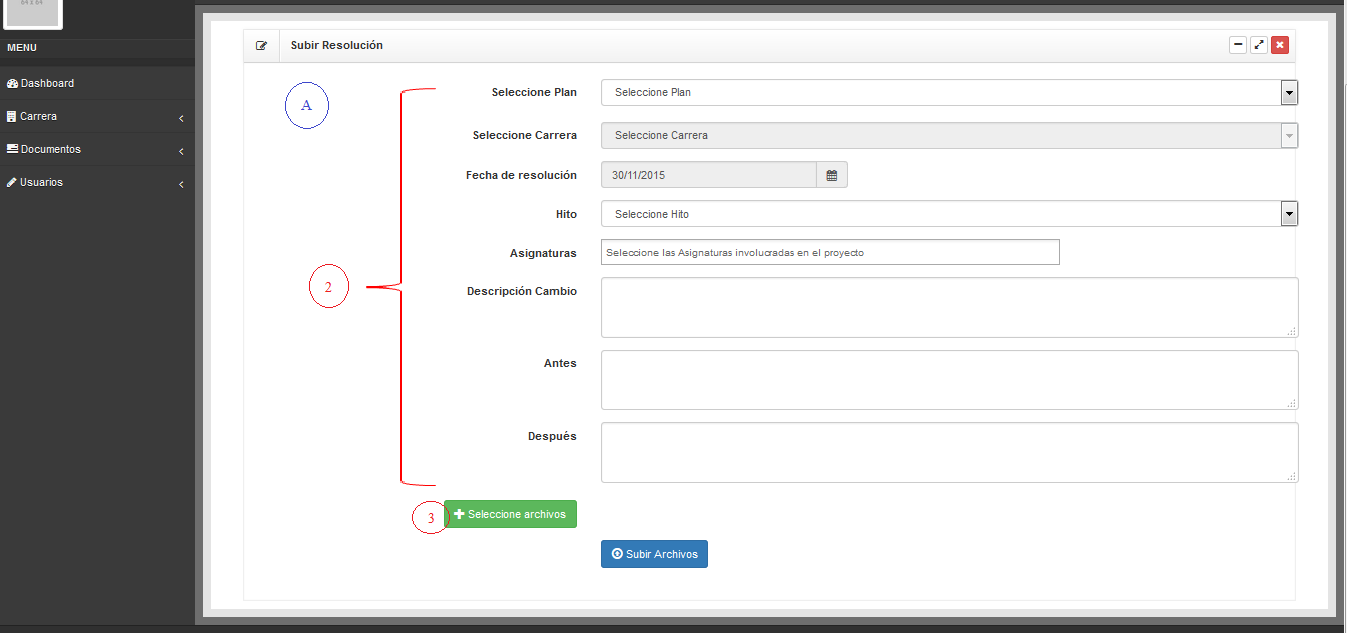
\includegraphics[width=1\textwidth]{images/Capitulo_3/subir_documento2.png}} \\ 
				
				\multicolumn{2}{c}{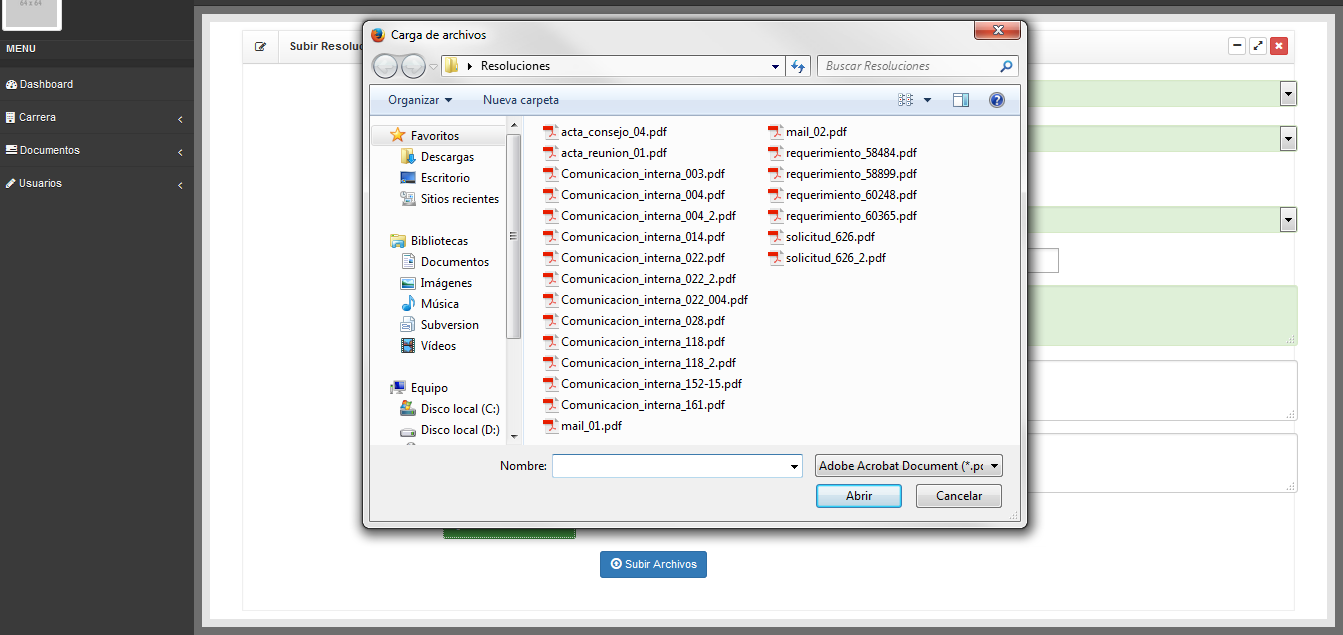
\includegraphics[width=1\textwidth]{images/Capitulo_3/subir_documento3.png}} \\ 
				
				\multicolumn{2}{c}{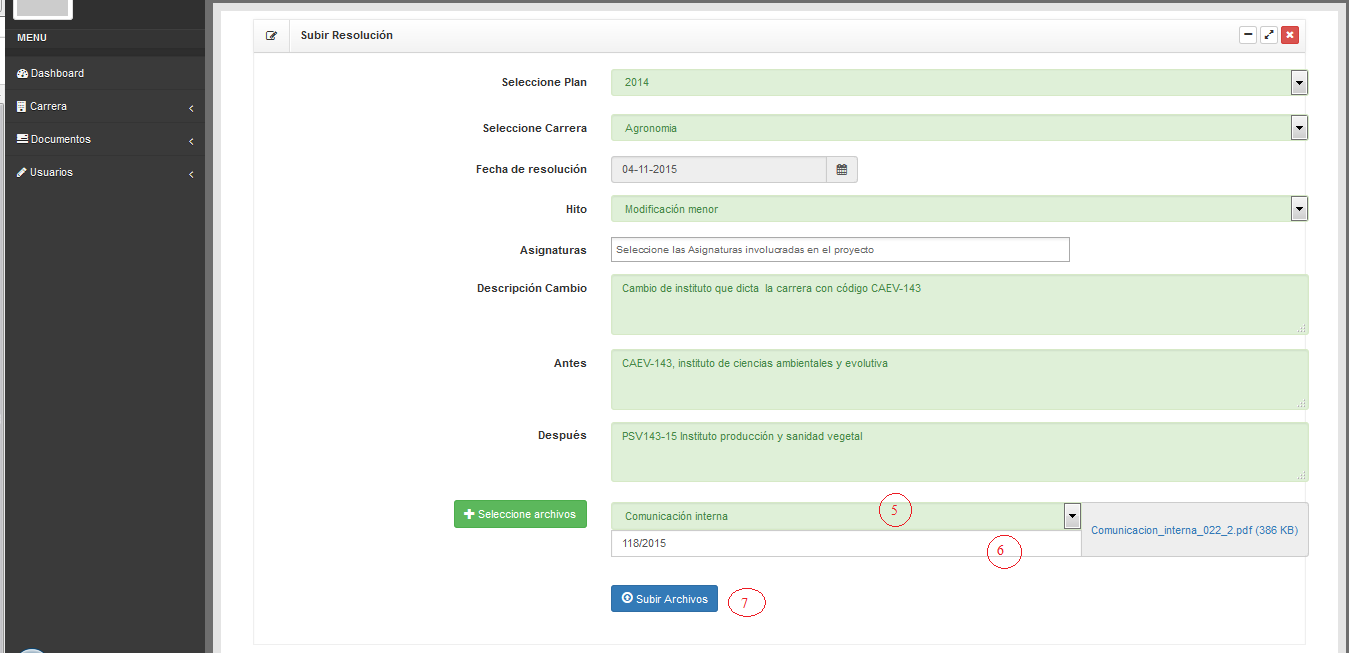
\includegraphics[width=1\textwidth]{images/Capitulo_3/subir_documento5.png}} \\ 
				
				
				\multicolumn{2}{c}{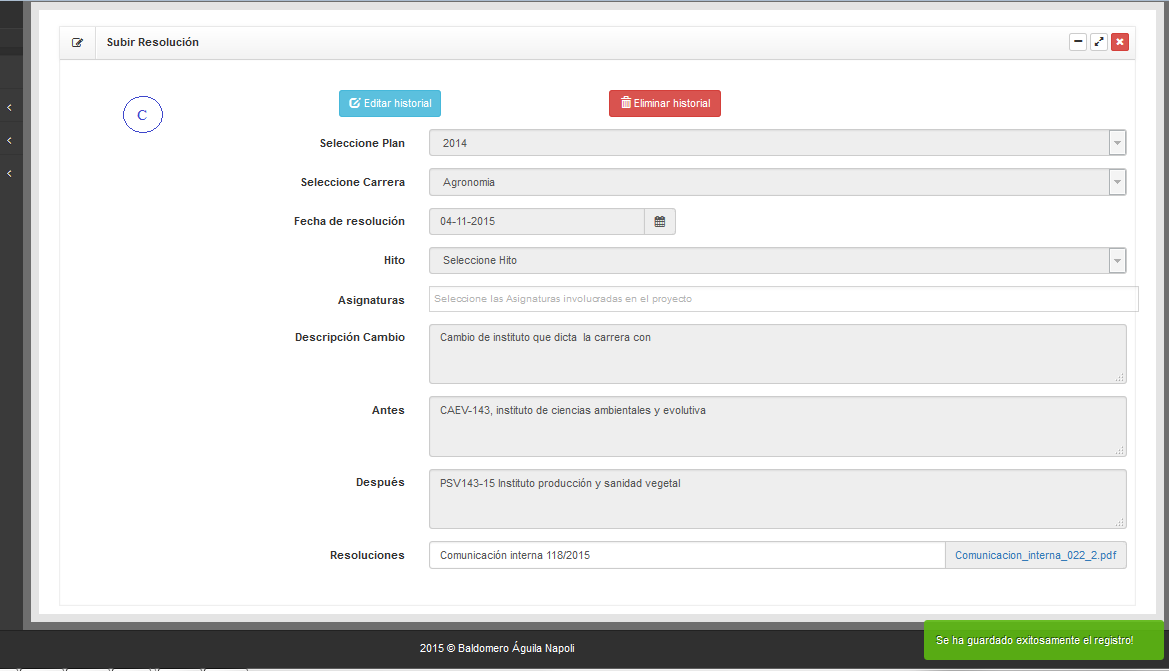
\includegraphics[width=1\textwidth]{images/Capitulo_3/subir_documento6.png}} \\ \hline
				
				\rowcolor{LightBlue2}  \multicolumn{2}{c}{Curso normal de eventos} \\ 
				
				\textbf{Acción actor} &	\textbf{Respuesta sistema} \\ \hline
				
				1.- Este caso de uso comienza cuando un usuario de tipo administrador y/o editor  desea crear un hito curricular, para ello debe hacer click en \textbf{1}.
				&	2.- El sistema despliega la pantalla \textbf{A}, el cual permite al usuario  introducir información referente al encabezado del hito curricular y subir documentos en formato pdf.\\ \hline
			
			
				3.- El usuario ingresa toda la información relacionada con el encabezado del hito curricular en \textbf{2}.
				& 4.- A medida que el usuario va completando los campos, el sistema va validando si están en el formato correcto, es decir, si la información debe ser del tipo: número, sólo letras, longitud máxima, longitud mínima, etc.\\ \hline
				
				5.- Una vez que el usuario haya introducido todos los campos requeridos por el sistema, procede a subir el o los documentos relacionados al hito, haciendo click en \textit{3}.
				& 6.- El sistema abre la ventana que se muestra en \textit{B}.\\ \hline
				
				7.- El usuario selecciona todos los archivos en formato pdf que desee subir, luego hace click en ``Abrir''.
				& 8.- Por cada documento que el usuario desee subir, el sistema  agregará a la interfaz gráfica los siguientes elementos; un DropDownList, en el cual el usuario selecciona el  tipo de documento qué es; un input, donde el usuario ingresa el número del documento y por último un Label que indica el nombre del documento.\\ \hline
				
				9.- El usuario completa los dos campos nuevos que se agregaron a la interfaz gráfica, para luego hacer clik en ``Subir Archivos''.
				& 10.- El sistema valida que los archivos estén en formato correcto.\\ \hline
				
			
				& 11.- El sistema recibe los datos del formulario y los almacena en la base de datos.\\ \hline
				
				& 12.- El sistema almacena la operación que se realizó (En este caso creación de un hito) en la bitácora de cambios del sistema. \\ \hline
				
				& 13.- El sistema redirecciona al usuario a la pantalla \textbf{C}. \\ \hline
				
				\rowcolor{LightBlue2}  \multicolumn{2}{c}{Curso alternativo de los eventos} \\ 
				
			
				& 10.- los archivos que el usuario intenta subir no están en formato pdf, o pesan más de 5 mb, por lo que el sistema muestra un mensaje de alerta y el usuario tiene que volver a la etapa Número 5.\\ \hline
				
			\end{longtable}
			
			


			
			En la Figura \ref{diagrama_secuencial_Subir_documento} se presenta el diagrama de secuencia para este mismo caso de uso, y así mostrar la interacción entre los distintos componentes del software que llevan a cabo esta tarea, a continuación se explicará el diagrama presentado.
			\begin{figure}[H]
				\centering
				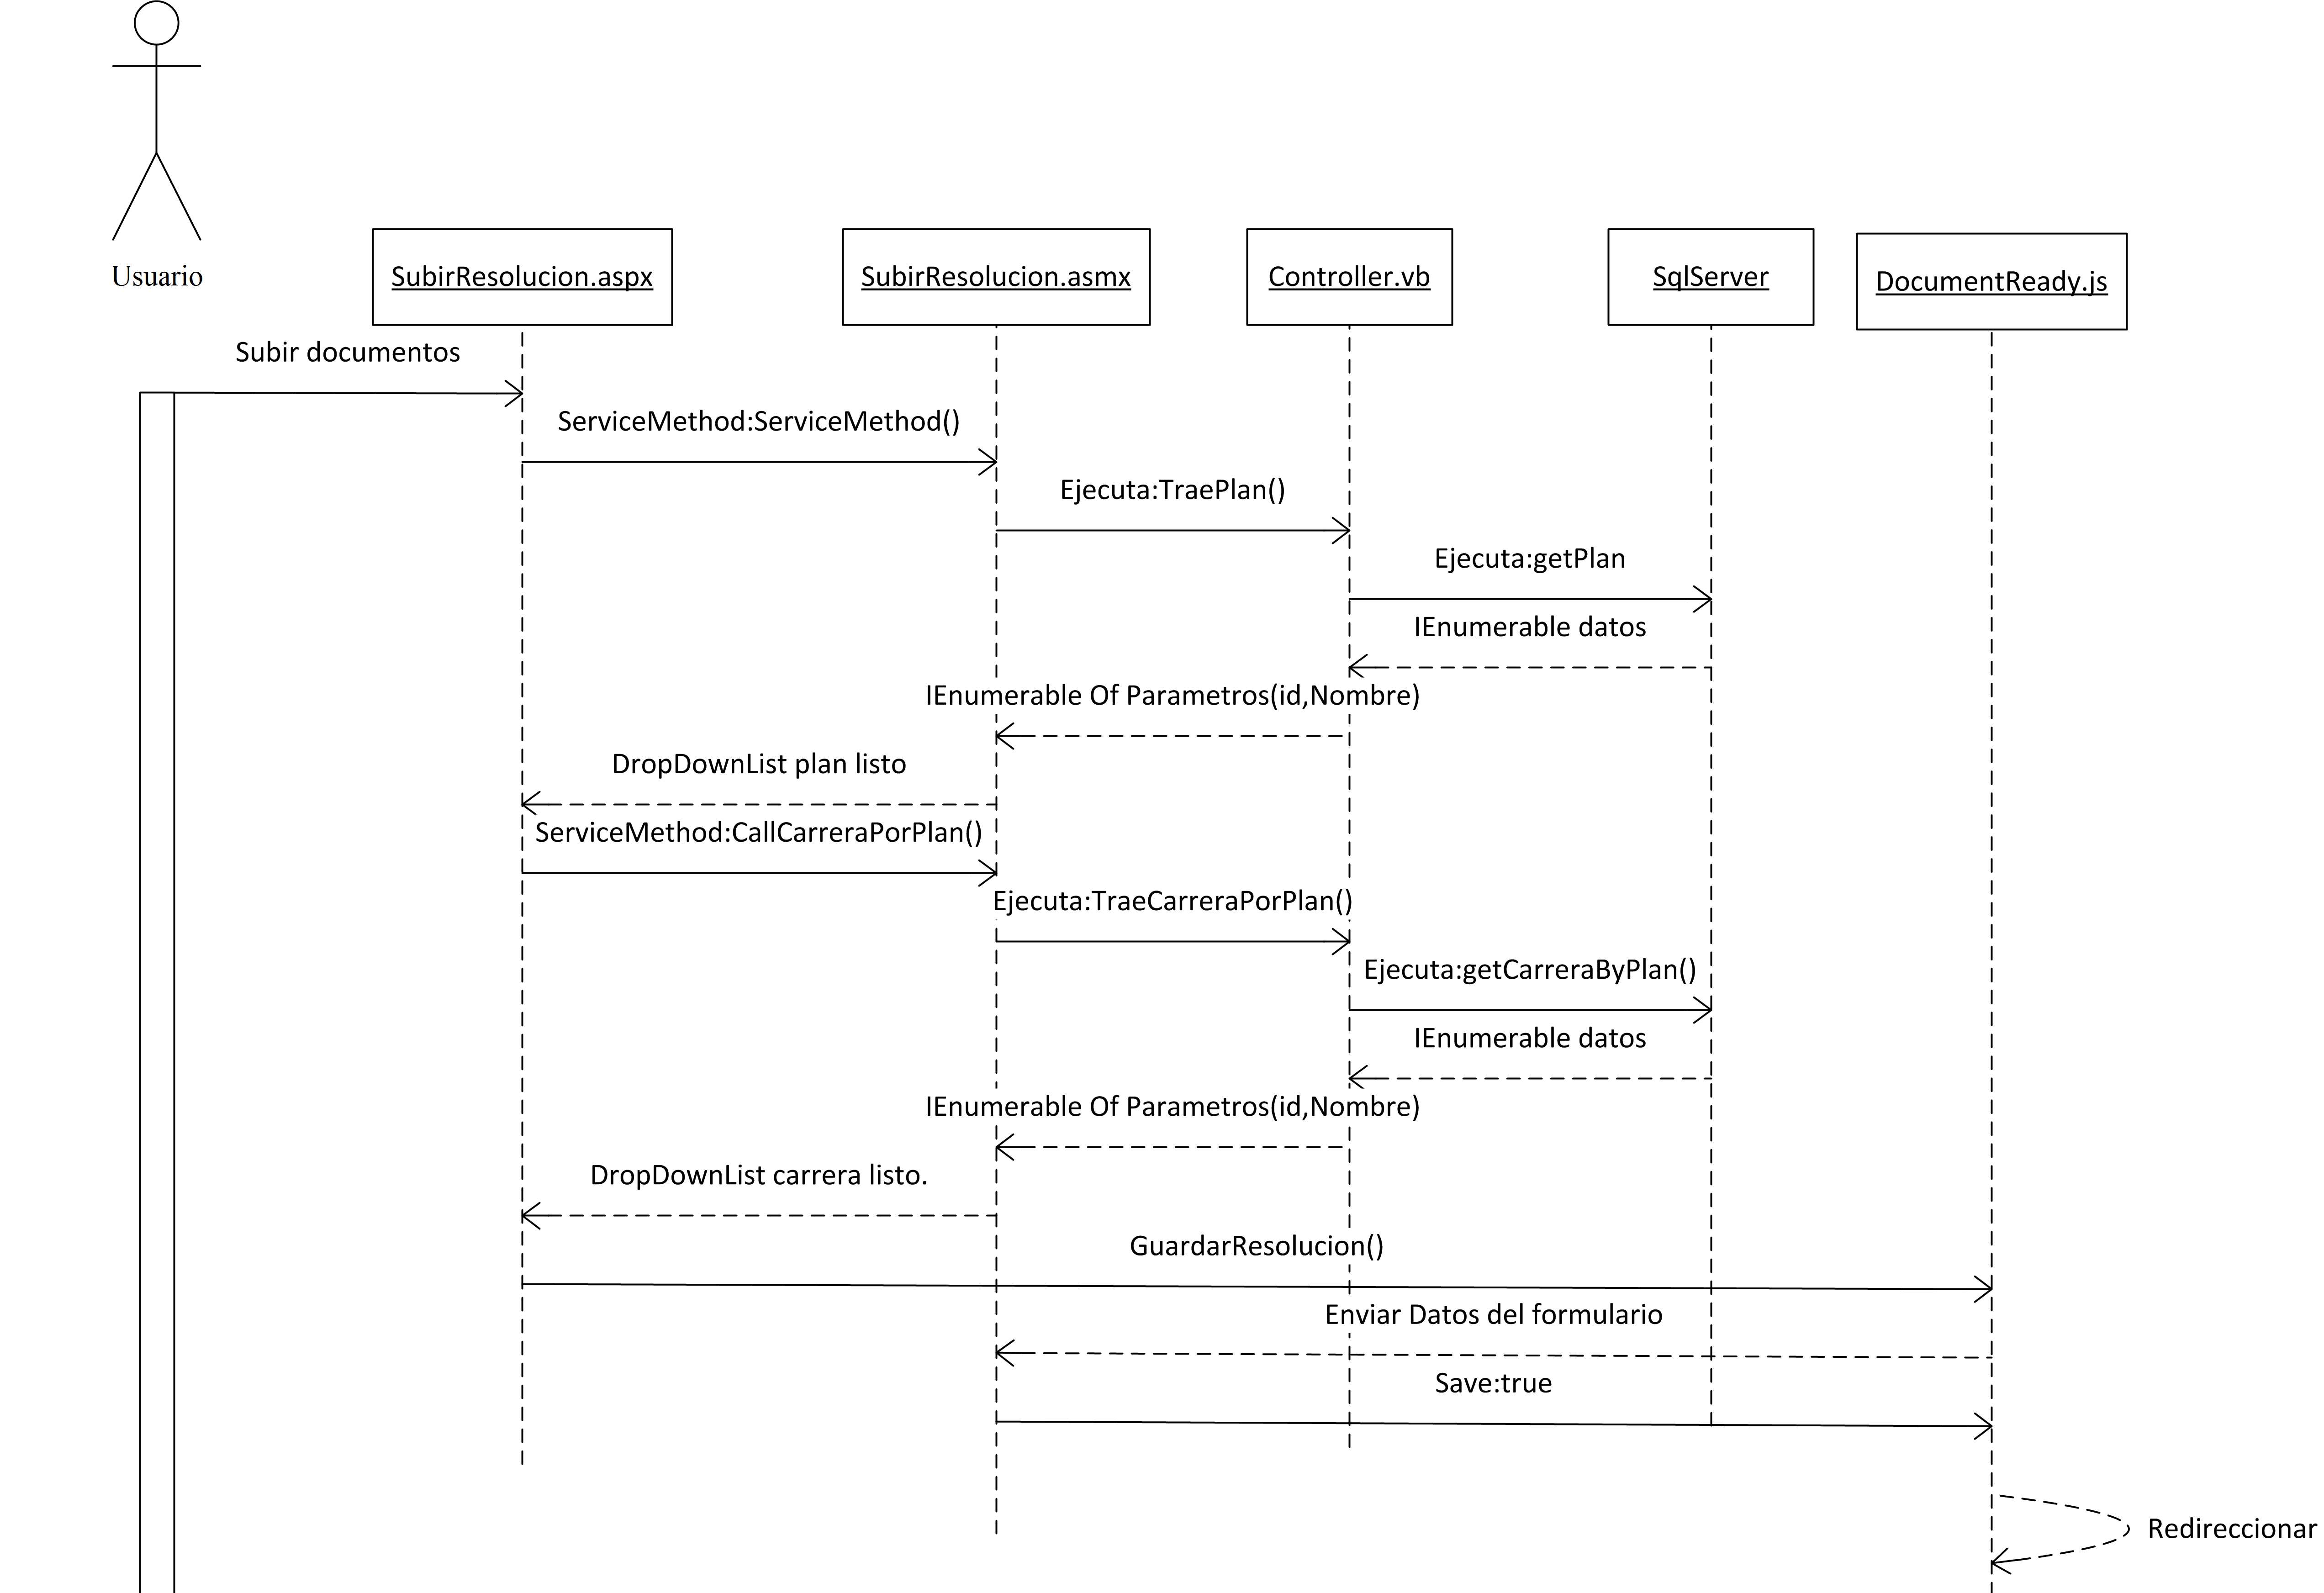
\includegraphics[width=1\textwidth]{images/Capitulo_3/Subir_Documentos.png}
				\caption[Diagrama de secuencia para el caso de uso \textit{Subir Documentos}]{Diagrama de secuencia para el caso de uso \textit{Subir Documentos} \footnote{}}
				\label{diagrama_secuencial_Subir_documento}
			\end{figure}
			\footnotetext{Elaboración propia.}
	
	
	Antes de describir el flujo de control de este caso de uso, hay que mencionar que el módulo Gestor de Documentos trabaja el poblado de los DropDownList del mismo modo que el módulo Historial Curricular, por lo que este proceso no se explicará  con mayor detalle en este diagrama.\\
	
	El flujo de este caso de uso comienza con la carga de la vista SubirResolución.aspx, para ello, antes de mostrar la vista al usuario que realizó la petición, se debe cargar previamente los elementos de las listas  desplegables correspondientes a: planes de estudios y asignaturas. Una vez   \textbf{probada las   listas  desplegables}( ver Sección \ref{Proceso_poblado_DDL} ) el sistema despliega el formulario para que el usuario lo manipule.\\
	
	Luego de que el usuario hay completado los campos necesarios, y haya seleccionado todos los archivos relacionados con el hito curricular que se desea crear, el usuario envía el mensaje \textbf{GuardarResolución} al componente DocumentReady.js, quien es el encargado de  enviar los datos del formulario mediante una petición POST al servicio web \textbf{SubirResolucion.asmx}.\\
	
	El flujo termina cuando el servicio web envía la variable Sabe:true al DocumentReady.js, con el fin de avisarle a este agente de que los cambios se almacenaron correctamente y que puede redireccionar al usuario a la vista de administración de los hitos curriculares.

	
	

	
	
	\mysubparagraph{ Caso de uso real del módulo gestor de documentos:``Ver documentos''} 
	
	El caso de uso ``Ver documentos'' corresponde al segundo caso de uso extendido del caso de uso  ``Gestor de Documentos''. en este caso de uso  todo usuario autentificado tiene acceso y ocurre cuando un  algún usuario quiere ver el repositorio de documentos que se encuentra en el sistema. El caso de uso real se presenta en la Tabla  \ref{Tabla_Caso_Uso_Ver_Documento}.
	
	\begin{longtable}{p{7cm}| p{7cm}}
		
		\caption{Caso de uso  Ver documentos}
		\label{Tabla_Caso_Uso_Ver_Documento}\\
		
		
		\hline
		\endfirsthead
		\multicolumn{2}{c}%
		{\tablename\ \thetable\ -- \textit{Continuación de la página anterior}} \\
		\hline
		
		\hline
		\endhead
		\hline \multicolumn{2}{r}{\textit{Continúa en la página siguiente}} \\
		\endfoot
		\hline \hline
		\endlastfoot
		\rowcolor{LightBlue2}  \multicolumn{2}{c}{Caso de uso  Ver documentos} \\  \hline
		
		
		\textbf{Actores} & Administrador, Editor y Suscriptor.\\ \hline
		
		\textbf{Propósito} & Visualizar el repositorio de documentos de los cambios curriculares de los planes de estudio.\\ \hline
		
		\textbf{Tipo} & Secundario y esencial\\ \hline
		
		\multicolumn{2}{p{15cm}}{\textbf{Resumen:} El administrador, editor o analista selecciona la sección correspondiente a  ver documentos, una vez seleccionado, el sistema  mostrará una tabla con todos los documentos de todas las facultades de la universidad. El usuario tendrá opciones de filtros para buscar ya sea por facultad, escuela, carrera y/o tipo de modificación.} \\  \hline \hline
		
		\rowcolor{LightBlue2}  \multicolumn{2}{c}{Interfaz: Formulario Ver Historial Curricular} \\  \hline \hline
		
		\multicolumn{2}{c}{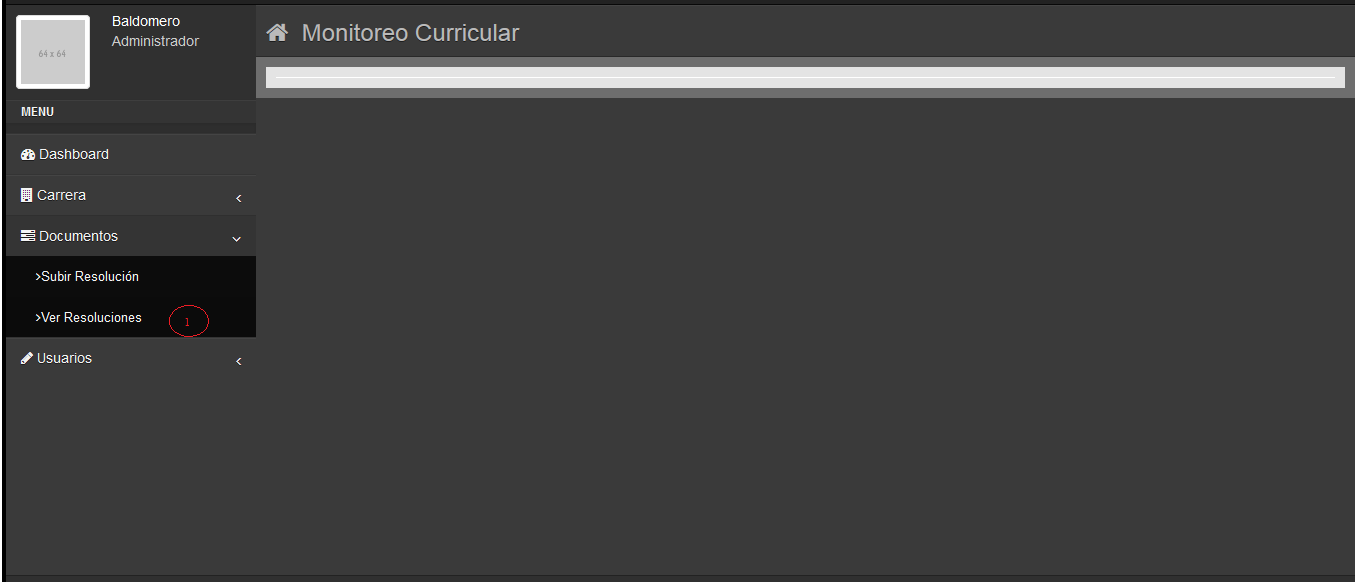
\includegraphics[width=1\textwidth]{images/Capitulo_3/VerDocumentos1.png}} \\ 
		
		\multicolumn{2}{c}{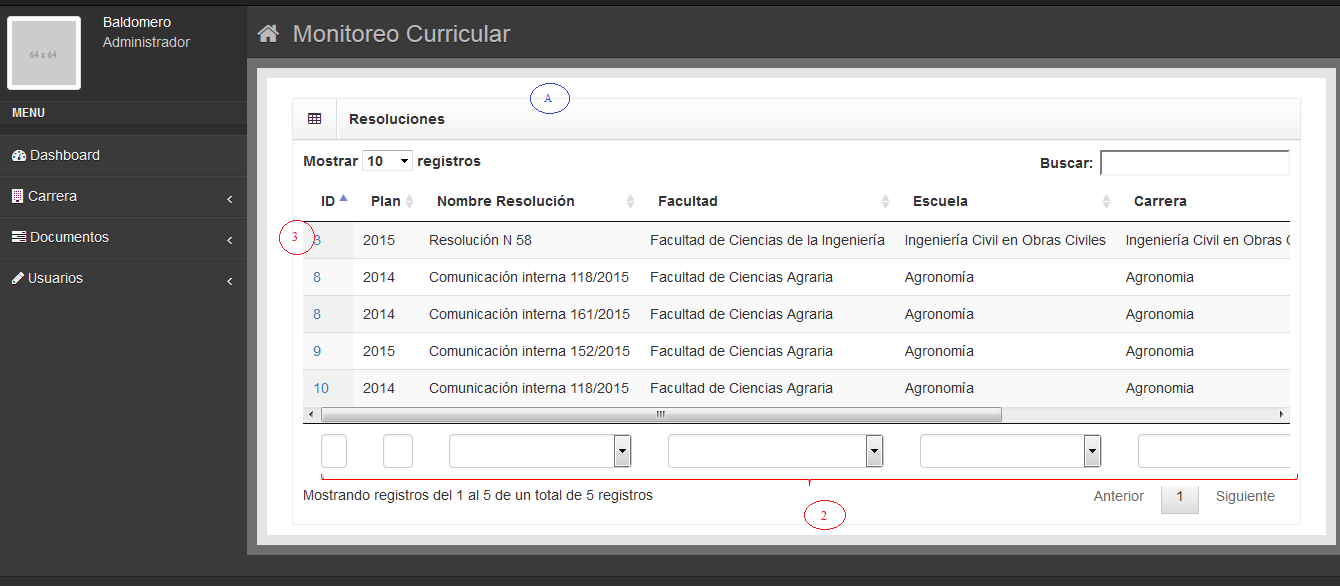
\includegraphics[width=1\textwidth]{images/Capitulo_3/VerDocumentos2.png}} \\ 
		
		\multicolumn{2}{c}{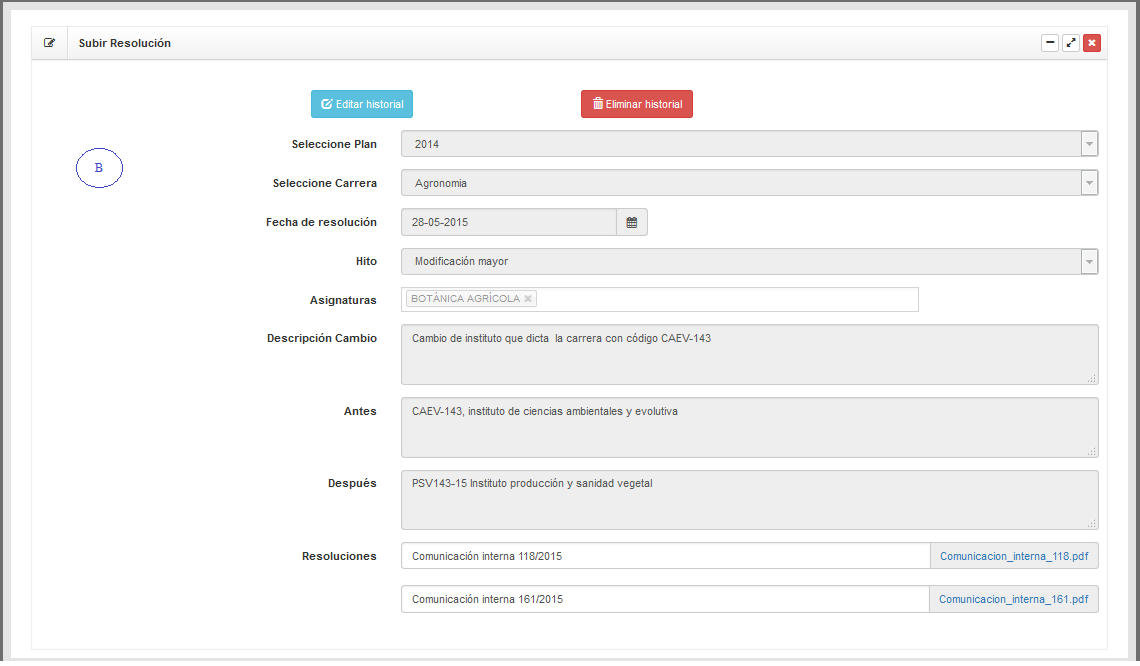
\includegraphics[width=1\textwidth]{images/Capitulo_3/VerDocumentos3.png}} \\  \hline
		
		\rowcolor{LightBlue2}  \multicolumn{2}{c}{Curso normal de eventos} \\ 
		
		\textbf{Acción actor} &	\textbf{Respuesta sistema} \\ \hline
		
		1.- Este caso de uso comienza cuando un usuario autentificado desea ver el repositorio de documentos, para ello debe hacer click en \textbf{1}.
		&	2.- El sistema despliega la pantalla \textbf{A}, el cual permite al usuario visualizar una tabla con el registro de los documentos.\\ \hline
		
		
		3.- El usuario puede hacer algún tipo de filtro avanzado utilizando los DropDownList que se muestran en \textbf{2}.
		& 4.- El complemento DataTable se  encarga de leer los filtros y reducir las filas de la tabla.\\ \hline
		
		5.- El usuario selecciona el hito que desea visualizar, para ello hace click en el id del registro( \textit{3}).
		& 6.- El sistema despliega el hito  con sus documentos en  la ventana que se muestra en \textit{B}.\\ \hline

	
	\end{longtable}
	
	
	
			En la Figura \ref{diagrama_secuencial_ver_documento} se presenta el diagrama de secuencia para este mismo caso de uso, y así mostrar la interacción entre los distintos componentes del software que llevan a cabo esta tarea, a continuación se explicará el diagrama presentado.
			\begin{figure}[H]
				\centering
				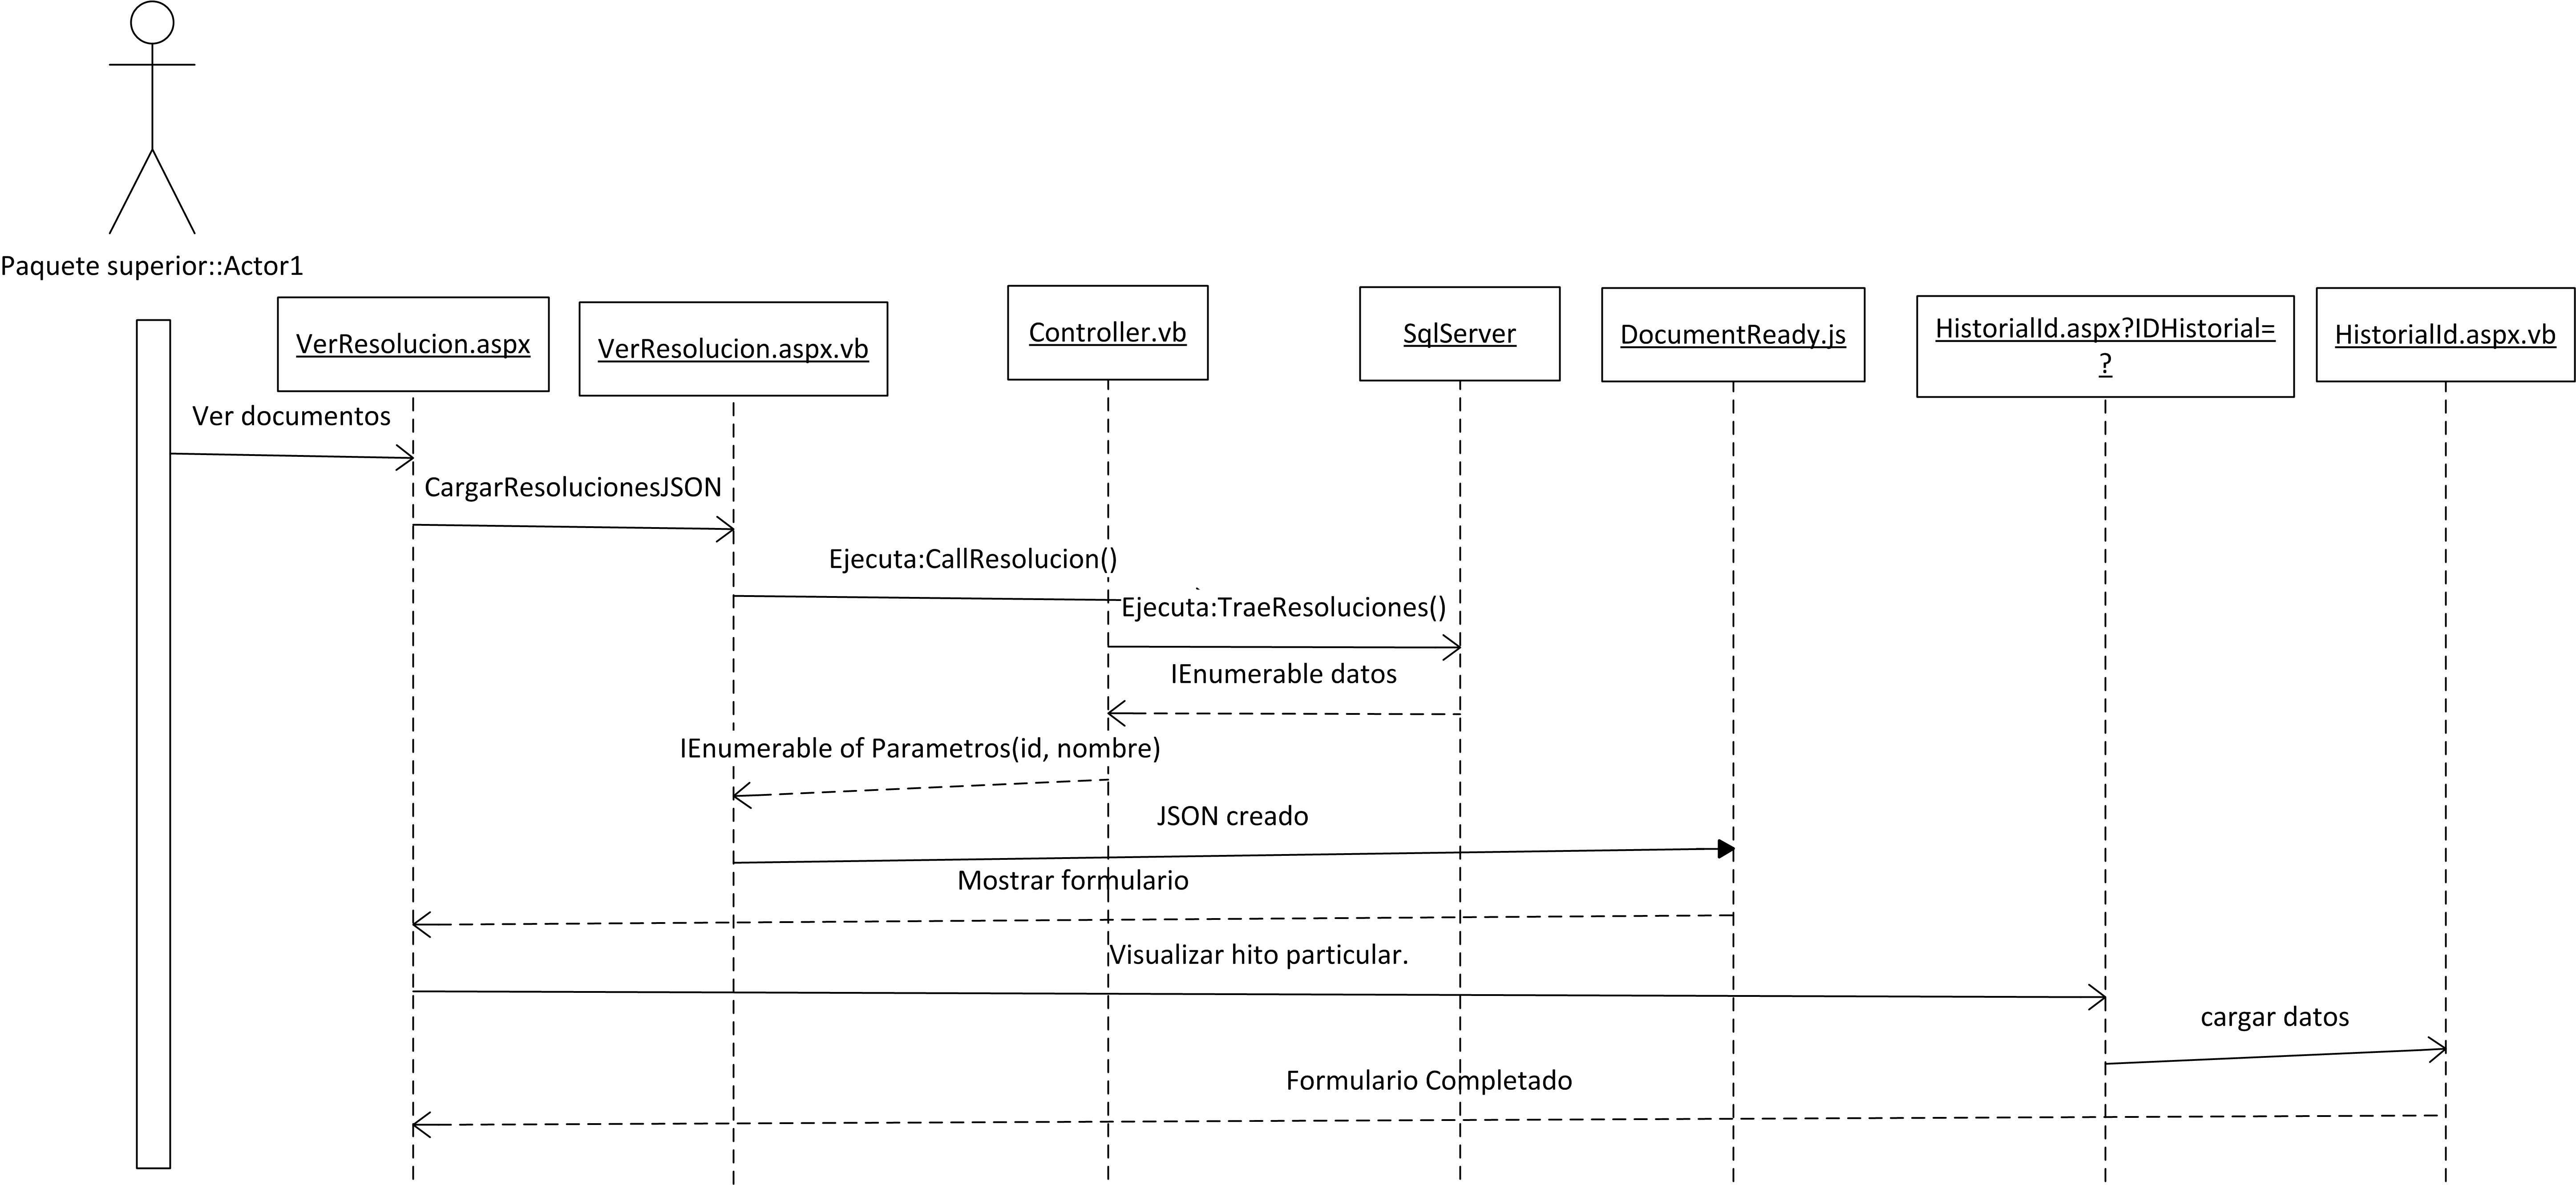
\includegraphics[width=1\textwidth]{images/Capitulo_3/ver_Documentos.png}
				\caption[Diagrama de secuencia para el caso de uso \textit{Ver Documentos}]{Diagrama de secuencia para el caso de uso \textit{Ver Documentos} \footnote{}}
				\label{diagrama_secuencial_ver_documento}
			\end{figure}
			\footnotetext{Elaboración propia.}
			

	Cuando un usuario autentificado desea ver algún documento almacenado en la base de datos (resolución, comunicación interna, decretos, etc.), la vista VerResolucion.aspx es la que comienza con toda la secuencia que permite que este caso de uso se ejecute satisfactoriamente.
	\\
	
	El primero lugar VerResolucion.aspx solicita los datos de todas las resoluciones a la biblioteca Controller.vb mediante la acción CallResolucion(), una vez que esta biblioteca reciba el mensaje, ejecuta el procedimiento almacenado TraeResoluciones().
	\\
	
	Una vez que la consulta se haya efectuado exitosamente, la biblioteca Controller tiene que dar formato a estos  datos obtenidos de la base de datos, para que posteriormente se envíen al \textit{code behind} \footnote{Archivo que contiene el código ejecutable de las vistas en ASP.NET} de la vista VerResolucion.aspx.
	\\
	
	Después de que la vista VerResolucion.aspx reciba los datos del Controller.vb, crea el Archivo JSON y se envía una variable JSON = true al agente DocumentReady.js. Al recibir la variable de éxito, DocumentReady.js se encarga de cargar los datos del archivo a la tabla y finalmente mostrar formulario final al usuario autentificado.









\newpage
%----------------------------------------------------------
%----------------------------------------------------------
\section{IMPLEMENTACIÓN}
Este capítulo describe las diferentes etapas por las que ha atravesado el desarrollo de
este sistema hasta llegar a su última iteración. Se inicia con una breve reseña de los pasos
previos al desarrollo, es decir, la instalación de herramientas y configuración de la máquina
de trabajo donde se desarrolló la aplicación web. Posteriormente se muestran los tres incrementos del prototipo del sistema.

\subsection{Configuración del ambiente de desarrollo}

Como se mencionó en la Sección \ref{SecReCNoF}, uno de los requisitos no funcionales es que el proyecto este programado con la estructura con la que trabaja la DTI, dado que el proyecto quedará funcionando en estas dependencias. Para llevar acabo este requisito, el alumno tesista tuvo aproximadamente cinco reuniones con Don Milton Muñoz, encargado del desarrollo y mantenimiento de sistemas y con la Sra. Paola Juarez Morales, encargada del Desarrollo de Sistemas. El propósito de estas reuniones se describen a continuación.
\\

En primero lugar fue necesario entender el contexto en el cual estaba inmerso el proyecto, por lo que fue necesario que Don Milton Muñoz facilitara todas las entidades de la base de datos de la Universidad que tenían relación directa con el sistema.
\\

Una vez entregado el modelo relacional, se procedió a instalar las herramientas necesarias para el desarrollo en el equipo de trabajo, las herramientas instaladas fueron:
\begin{itemize}
	\item Microsoft Visual Studio Professional 20013
	\item Microsoft SQL Server 2008 R2
\end{itemize}

Durante la instalación de las herramientas mencionadas no hubo mayores problemas.
\\

Finalmente, en conjunto con la Sra. Paola, el alumno tesista creó el ``esqueleto'' de la plataforma web, el cual estaba separa por las 3 capas de negocio (aplicación web, biblioteca de clases y biblioteca de servicios WCF) y además se realizó la configuración de la conexión a la base de datos.



\subsection{Consideraciones Técnicas}

Esta sección describe los elementos necesarios para que el sistema funcione de manera óptima:

\begin{itemize}
	\item alertify v0.3.11
	\item Metis - Bootstrap-Admin-Template v2.3.2
	\item daterangepicker v1.3.22
	\item jQuery  bpopup v0.11.0
	\item DataTables v1.10.7
	\item jQuery wizard plug-in v3.0.7
	\item jQuery Input Limiter plugin v1.3.1
	\item jQuery Rut v0.5
	\item jQuery Validation Plugin v1.14.0
	\item jQuery validVal v5.0.2
	\item Parsleyjs v2.2.0-rc1
	\item Visual Basic 2013
	\item Sql Server 2008 R2\end{itemize}


\subsection{Dificultades de la implementación} \label{Dificultades}



Una de las principales dificultades que se presentó al momento de desarrollar la aplicación, fue el trabajar con una arquitectura orientada a servicios, si bien este paradigma esta siendo usado por la mayoría de las aplicaciones web distribuidas, el alumno  tesista no tenia experiencia en este tipo de programación, por lo que antes de programar todos los servicios web necesarios para el buen funcionamiento de la aplicación, el alumno tesista tuvo que leer sobre esta paradigma, y esto entorpeció bastante el comienzo del desarrollo.\\

Otra dificultad detectada mientras se desarrollaba la aplicación, fue entender el paradigma de desarrollo de ASP.NET, en vista de que al usar \textit{code behind}, ASP.NET utiliza sus propios controles, y  al momento de compilar, estos controles se transforman en elementos HTML. Así, por ejemplo, el control \textit{DropDownList} de ASP.NET es equivalente a la etiqueta HTML \textit{select}. El trabajar con estos tipos de  controles hace que ciertas peticiones (GET, POST, PUT, etc.) se efectúen de forma diferente, y como se mencionó anteriormente, el alumno no poseía ni conocimientos ni experiencia en la la forma en la que trabaja ASP.NET.
\\

ASP.NET trabaja con la variable \textit{IsPostBack}, el cual nos entrega un valor que indica si la página se está cargando como respuesta a un valor devuelto por el cliente, o si es la primera vez que se obtiene acceso a ella. Esto ocasionó  problemas con alguno de los plugins que se incorporaron  al proyecto, como por ejemplo el sistema de notificaciones(alertify.js), el cual utiliza un una etiqueta \textit{div} como un  \textit{popUp} para mostrar un \textit{alert} modificado. Al principio se pensó que el sistema de notificaciones no funcionaba correctamente, ya que los valores de las alertas no se almacenaban, sin  embargo después de depurar las acciones sobre las alertas con Firebug, se verificó que el problema no era de plugin, si no que era de la variable \textit{isPostBack}.
\\

En cuanto a la base de datos, el único problema que hubo, fue el tratar de dar un correcto formato a la salida de los procedimientos almacenados. En principio el retorno de los procedimientos era  un \textit{1} si el procedimiento se ejecutaba correctamente, o un \textit{-1} si no se ejecutaba, sin embargo este tipo de codificación era bastante ambigua, ya que si salía un \textit{-1}, no se sabia que tipo de error había ocurrido en el sistema, a si que se procedió a trabajar en una codificación 
 mucho más precisa.
\\

Por último, hay que mencionar que una de las tareas  que presentó complicaciones, fue la depuración de la aplicación, y esto ocurrió a causa de que las salidas de los procedimientos y servicios web no estaban estandarizados, y al momento de depurar la aplicación no se sabia con exactitud en que sección del código habia ocurrido la excepción.
\\

En resumen las mayores dificultades se presentaron en el desconocimiento de las tecnologías utilizadas.


\subsection{Presentación de prototipos}

El propósito de esta sección, es mostrar el crecimiento del sistema en las diferentes iteraciones. En cada incremento se describen los pasos que efectuaron para finalizar con la iteración exitosamente.




\newpage
%----------------------------------------------------------
%----------------------------------------------------------
\section{VALIDACIÓN DE LA PLATAFORMA}
Las pruebas que serán mostradas en este último capítulo, corresponden a una demostración funcional del sistema web.
se efectuarán distintas pruebas con el objetivo de verificar  el correcto funcionamiento de todos los requisitos funcionales descritos en el Capítulo \ref{Desarrollo_Sistema}.
\subsection{REQF-01: Autentificación de usuario}


En la Figura \ref{REQF-01} se muestra el inicio de sesión, los campos son: R.U.N del usuario y
Contraseña,


	\begin{figure}[H]
		\centering
		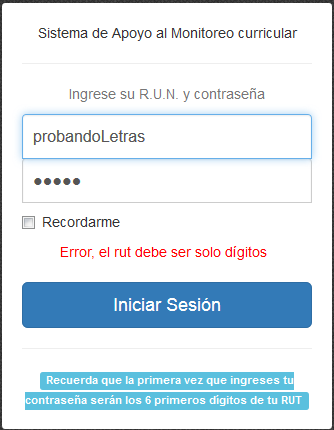
\includegraphics[width=0.5\textwidth]{images/Capitulo_5/REQF-01.png}
		\caption[REQF-01: Autentificación de usuario]{REQF-01: Autentificación de usuario \footnote{}}
		\label{REQF-01}
	\end{figure}
	\footnotetext{Elaboración propia.}
	
	
	Se realizaron distintas pruebas para comprobar el correcto funcionamiento de este requisito. A continuación se describen las distintas pruebas realizadas:
	\begin{itemize}
		\item Validación de números: El nick del usuario es su R.U.N. sin el dígito verificador, por lo que el sistema tiene que validar si el usuario ingresa cualquier carácter que no corresponda a un dígito. En caso de que el usuario ingrese algún carácter que no sea dígito, el sistema muestra el siguiente mensaje: \textbf{Error, el rut debe ser solo dígitos.}
		
		\item Validación nula: Los  dos campos solicitados  este formulario son campos obligatorios, por lo que si el usuario hace click en iniciar sesión y no ha completado estos campos, el sistema muestra un mensaje de alerta, impidiendo que el servidor realice cálculos innecesarios. Esta validación se ilustra en la Figura \ref{REQF-01-null}.
	\end{itemize}
	
	\begin{figure}[H]
		\centering
		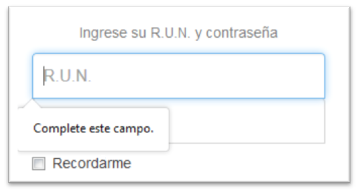
\includegraphics[width=0.7\textwidth]{images/Capitulo_5/REQF-01-null.png}
		\caption[REQF-01: Autentificación de usuario, validación de campos nulos]{REQF-01: Autentificación de usuario, validación de campos nulos}
		\label{REQF-01-null}
	\end{figure}
	
\subsection{REQF-02: Gestión de perfil}

\begin{figure}[H]
	\centering
	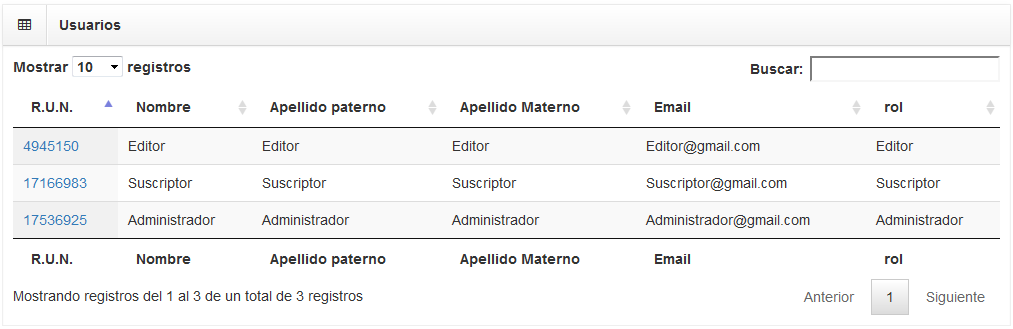
\includegraphics[width=1\textwidth]{images/Capitulo_5/REQF-02.png}
	\caption[REQF-02: Gestión de perfil]{REQF-02: Gestión de perfil}
	\label{REQF-02}
\end{figure}

La Figura \ref{REQF-02} ilustra la gestión de perfiles del sistema,  este requerimiento solo puede ser accedido por un usuario de tipo administrador.
\\
En primer lugar se realizaron pruebas para comprobar que los usuarios del tipo Editor y Suscriptor  no tuvieran acceso, para ello se crearon  tres usuarios con los tres tipos de perfiles existentes, con el fin de autentificarse y tratar de acceder a este requisito. los resultados muestran en la Tabla \ref{pruebas_gestionPerfiles}.

\newpage
	\begin{longtable}{l |l}
		
		\caption{Resultados de pruebas del acceso a la gestión de perfiles}
		\label{pruebas_gestionPerfiles}\\
		
		
		\hline
		\endfirsthead
		\multicolumn{2}{c}%
		{\tablename\ \thetable\ -- \textit{Continuación de la pagina anterior}} \\
		\hline
		
		\hline
		\endhead
		\hline \multicolumn{2}{r}{\textit{Continúa en la página siguiente}} \\
		\endfoot
		\hline
		\endlastfoot
		\rowcolor{LightBlue2} Tipo de perfil & Resultado de acceso\\ \hline
		
		Administrador & Se pudo acceder exitosamente.\\ \hline
		
		Editor & No se pudo acceder.\\ \hline
		
		Suscriptor & No se pudo acceder.\\ \hline \hline
	\end{longtable}

En segundo lugar se realizaron pruebas para las siguientes operaciones básicas de este requisito: Actualizar usuario y Eliminar usuario. el proceso y los resultados de cada prueba se detallan a continuación.

\mysubparagraph{Actualizar usuario}

Uno de los Errores encontrados al momento de validar esta acción, fue que al tratar de actualizar  un usuario en particular  los datos que se enviaban mediante la petición POST al servidor no eran los correctos. El error detectado se puede apreciar gráficamente en las Figuras \ref{REQF-02-actualizar} y \ref{REQF-02-post}.


\begin{figure}[H]
	\centering
	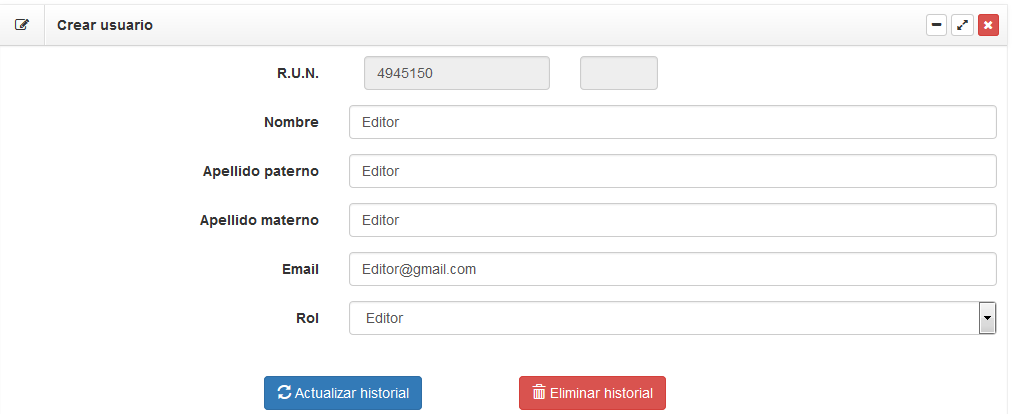
\includegraphics[width=1\textwidth]{images/Capitulo_5/REQF-02-agregar1.png}
	\caption[REQF-02: Gestión de perfil, Actualizar usuarios]{REQF-02: Gestión de perfil, Actualizar usuarios}
	\label{REQF-02-actualizar}
\end{figure}

Aunque el usuario autentificado esta intentando editar el  R.U.N. 4.945.150, en la Figura \ref{REQF-02-post}  se puede apreciar que, entre las variables que se están enviando, esta la variable Rut, que corresponde al R.U.N. editado, sin embargo el valor que esta tomando la variable  Rut no corresponde al R.U.N. editado, si no  que se esta enviando el R.U.N. de la persona autentificada. Este error fue corregido a tiempo.
\begin{figure}[H]
	\centering
	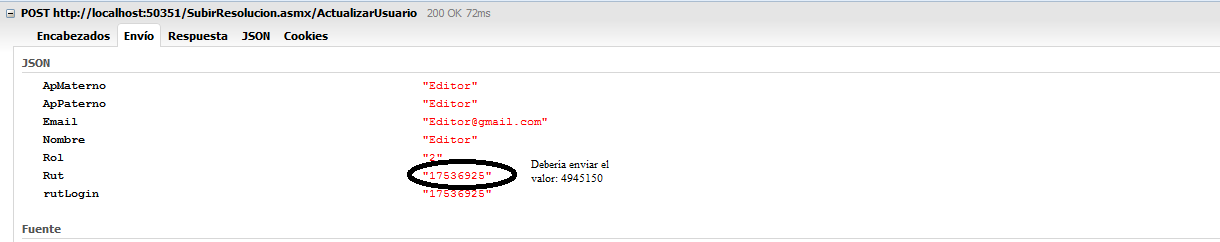
\includegraphics[width=1\textwidth]{images/Capitulo_5/REQF-02-post.png}
	\caption[REQF-02: Gestión de perfil, depuración de los datos enviados mediante la petición POST]{REQF-02: Gestión de perfi, depuración de los datos enviados mediante la petición POST}
	\label{REQF-02-post}
\end{figure}

\mysubparagraph{Eliminar usuario}

Comprobar el correcto funcionamiento del mensaje de alerta que se muestra en la Figura \ref{REQF-02-eliminar} era el principal objetivo de la validación de esta acción, ya que como se mencionó en la Sección \ref{Dificultades}, ASP.NET trabaja de una forma particular las peticiones POST de complementos externos.
\begin{figure}[H]
	\centering
	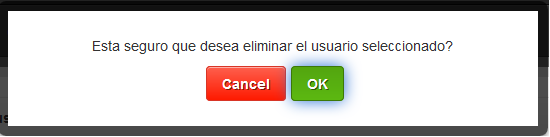
\includegraphics[width=1\textwidth]{images/Capitulo_5/REQF-02-Eliminar.png}
	\caption[REQF-02: Gestión de perfil, Mensaje de verificación para eliminar algún usuario]{REQF-02: Gestión de perfi, Mensaje de verificación para eliminar algún usuario}
	\label{REQF-02-eliminar}
\end{figure}

La verificación de esta acción se realizó mediante eliminaciones de registro. Se comprobó que los botones de la alerta generada(``Cancel'' y ``Ok'') realizaran sus respectivas acciones, además, se verificó de que si el registro eliminado poseía algún documento, éste fuera eliminado del servidor.


\subsection{REQF-03: Desplegar historial curricular}

Este requerimiento no necesitó mayores pruebas puesto que es un requerimiento de visualización.

\subsection{REQF-04: Registro de usuarios}

Uno de los datos que NO se pueden modificar una vez que se haya creado el usuario, es el R.U.N., por lo que es de vital importancia que este dato se ingrese correctamente al momento de registrar al usuario, para ello se consideró validar la existencia del R.U.N. ingresado mediante el plugins jQuery.Rut.js. \\

En caso de que el R.U.N. ingresado no existiera el sistema muestra gráficamente un mensaje de que el R.U.N. no existe (Ver Figura \ref{REQF-02-rut}), impidiendo que el usuario se almacene en la base de datos.

\begin{figure}[H]
	\centering
	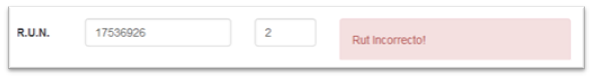
\includegraphics[width=1\textwidth]{images/Capitulo_5/REQF-02-rut.png}
	\caption[REQF-02: Gestión de perfil]{REQF-02: Gestión de perfil}
	\label{REQF-02-rut}
\end{figure}

Con respecto a los demás campos se validó que todos los campos sean obligatorios y que el formato del correo electrónico sea un formato  válido.


\subsection{REQF-05:Gestión de documentos}

Se realizaron distintas pruebas para comprobar el correcto funcionamiento de este requisito. A continuación se describen las distintas pruebas realizadas:
\begin{itemize}
	\item Validación nula: Todos los  campos solicitados en  este formulario son campos obligatorios, por lo que si el usuario deja un campo sin completar, y luego  hace click en Subir archivos, el sistema de forma inmediata marca en rojo todos los campos que no se han completado, y le informa al usuario de que son campos obligatorios.
	
	\item Validación de Formato de archivos: Se intentó subir archivos de distintos formatos (.jpg, word, ppt, etc) y el resultado que el sistema muestra un mensaje de Alerta indicando que el formato no es el correcto (Ver Figura \ref{REQF-05} ).
	
	\item Validación de eliminación de archivos: Se eliminaron registros curriculares con el fin de verificar que el registro se eliminara en su totalidad del sistema, es decir, que se eliminaran el registro en la base de dato y que se eliminara los archivos vinculados a ese registro eliminado del servidor.
\end{itemize}


\begin{figure}[H]
	\centering
	
\includegraphics[width=0.5\textwidth]{images/Capitulo_5/REQF-05.png}
	\caption[REQF-05: Gestión de documentos, Mensaje de alerta ]{REQF-05: Gestión de documentos, Mensaje de alerta }
	\label{REQF-05}
\end{figure}
\subsection{REQF-06:Visor de PDF}

Este requerimiento no necesitó mayores pruebas puesto que es un requerimiento de visualización.

\subsection{REQF-07:Notificaciones}


Este requisito se validó en conjunto con los demás requisitos, ya que el sistema de notificaciones esta presente en todo el sistema.
\\

Básicamente el usuario se cercioró de que el sistema de alertas este presente cuando un usuario autentificado realizara alguna operación sobre los datos del sistema.
\\

 En la Figura \ref{REQF-07} se muestra un ejemplo de una notificación exitosa.
 
\begin{figure}[H]
	\centering
	
\includegraphics[width=0.5\textwidth]{images/Capitulo_5/REQF-07.png}
	\caption[REQF-07: Notificaciones, alerta exitosa ]{REQF-07: Notificaciones,alerta exitosa }
	\label{REQF-07}
\end{figure}

A  pesar de que el sistema de notificaciones esta presente en toda la plataforma, éste requisito fue casi uno de los últimos en ser programados, a causa de esto, hubieron muchas acciones que NO tenían su alerta activa.

\subsection{REQF-08:Almacenar bitácora de los usuarios}


El objetivo de este requisito es facilitar la identificación  de la localización de los errores del sistema, por lo que es de vital importancia su correcto funcionamiento.\\

La validación de este requerimiento es muy distinta a todas las otras validaciones, ya que las validaciones anteriores dependían de los mensajes de alerta que el sistema entregaba, mientras que la validación de este requerimiento depende estrictamente de las salidas de los procedimientos almacenados de la base de datos y de las salidas de los servicios web del sistema, a causa de esto, el alumno tesista se enfocó en validar  los procedimientos y los servicios web. Las distintas pruebas realizadas se describirán a continuación.
\\

En primer lugar, el alumno tuvo que validar que las salidas de todos los procedimientos sean estándar, puesto que las salidas se almacenan en la tabla REGISTRO, y esta tabla posee  campos obligatorios. El proceso de validación se realizó mediante la ejecución de los procedimientos almacenados y la lectura de las salidas de estos mismos en la consola de SQL Server. Los campos de las salidas de los procedimientos que producen cambios en el sistema son los siguientes:


\begin{itemize}
	\item \textbf{ErrorNumber:} Identificador único del mensaje.
	\item \textbf{ErrorMessage:} Descripción del mensaje.
	\item \textbf{ErrorDate:} Fecha en la que ocurrió en evento.
\end{itemize}

Una vez  validados los procedimientos, se procedió  a validar los servicios web, para ello fue de gran ayuda el complemento Firebug, ya que el Alumno validó las salidas de los servicios, mediante textos enviados  a la consola de Firebug. En la Figura \ref{REQF-09}, se puede apreciar una salida de un mensaje de error de un servicio web.

\begin{figure}[H]
	\centering
	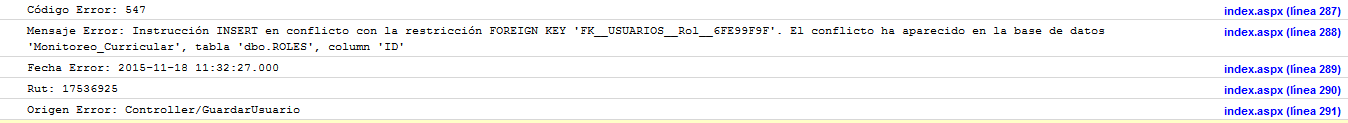
\includegraphics[width=1\textwidth]{images/Capitulo_5/REQF-09.png}
	\caption[REQF-09: Almacenar bitácora de los usuarios, salida de un procedimiento. ]{REQF-07: Almacenar bitácora de los usuarios, salida de un procedimiento. }
	\label{REQF-09}
\end{figure}
\subsection{REQF-09:Visualización de bitácora}

Este requerimiento no necesitó mayores pruebas puesto que es un requerimiento de visualización.


\newpage
%----------------------------------------------------------
%----------------------------------------------------------
\section{CONCLUSIONES}
La Universidad Austral de Chile se encuentra en una etapa de cambios dado que ya ha empezado con
el proceso de innovación curricular.  Inicialmente la documentación de estos procesos curriculares  se ha almacenado en distintos medios y en varias unidades de la organización. Al comienzo, este modo de gestión  funcionó relativamente bien, sin embargo, a  medida que el número de carreras innovadas fue creciendo,  este tipo de administración  fue retrasando la gestión de procesos estratégicos de seguimiento y auto evaluación.
\\


El desarrollo del presente proyecto  pretende apoyar la gestión de los procesos curriculares de estudios de pregrado, y como queda en evidencia en el  capítulo \ref{Desarrollo_Sistema}, el objetivo general se ha cumplido en su totalidad.
\\

El sistema no solo permite tener un historial de cambios curriculares en los planes de estudio, si no también permite el almacenamiento centralizado de los documentos relacionados con estos procesos, lo cual permite  que la documentación no se deteriore con el tiempo, y también disminuye el tiempo de búsqueda de estos mismos.\\

Una de las dificultades iniciales identificados por el autor, fue el desarrollar una aplicación con tecnologías totalmente desconocidas para él. Es verdad que si no hubiera existido esta restricción, no hubiera habido mayores dificultades, sin embargo, el trabajar con tecnologías desconocidas, fue un desafío que se propuso el estudiante para así al finalizar la tesis tener una retroalimentación de qué se siente trabajar bajo presión y sumarle el poco conocimiento sobre las herramientas de desarrollo.
\\ 


La  etapa de ``Validación'' del proyecto, es muy imporatante, ya que es inevitable que el sistema inicialmente no falle, puesto que al momento de programar existen muchos factores que hacen que el desempeño de la aplicación no sea el deseado, como por ejemplo  el cansancio, el estrés, entre otros factores. Gracias a esta etapa se pudo corregir a tiempo varios errores que se presentaron al momento de  probar la aplicación con datos reales.
\\



En Síntesis, en el contexto de la educación superior y del cambio de paradigma en el modelo educativo que busca implementar la universidad, esto es, pasar de un modelo centrado en la enseñanza (profesor) a uno centrado en el aprendizaje (estudiante), es importante que las unidades encargada de administrar estos procesos posean un sistema informático que facilite no solo la búsqueda de documentos, si no también  que almacene la trayectoria de los planes de estudios con el objetivo de tener una referencia de cambios.




\subsubsection{Trabajo futuro}
El paso siguiente es la integración total del software desarrollado con los sistemas de la Universidad, para ello se elaboró una propuesta de trabajo, la cual se puede ver en la Tabla \ref{Tabla_Propuesta_trabajo}.


	\begin{longtable}{l|p{7cm} |p{4cm}}
		
		\caption{Propuesta de trabajo}
		\label{Tabla_Propuesta_trabajo}\\
		
		
		\hline
		\endfirsthead
		\multicolumn{3}{c}%
		{\tablename\ \thetable\ -- \textit{Continuación de la pagina anterior}} \\
		\hline
		
		\hline
		\endhead
		\hline \multicolumn{3}{r}{\textit{Continúa en la página siguiente}} \\
		\endfoot
		\hline
		\endlastfoot
		
		\rowcolor{LightBlue2} Nombre hito & Descripción & Actores\\ \hline
		Reunión &
		Coordinar una reunión con el encargado de desarrollo de la DTI para  crear un ambiente de desarrollo con el fin de que el alumno tenga acceso a los datos reales de la universidad & 
		Alumno tesista, Patrocinante,Encargado de desarrolo de la DTI.\\ \hline
		
		Integración &
		El alumno tesista tiene que integrar en su totalidad el sistema desarrollado en el ambiente de desarrollo & 
		Alumno tesista.\\ \hline
		
		Reunión &
		Coordinar una reunión formar con Registro académico, con el fin de que este departamento provea documentación referente a los cambios curriculares & 
		Alumno tesista, Patrocinante, Jefa y secretaria  de Registro Académico.\\ \hline
		
		Documentación &
		Toda la información entregada por registro académico, se debe entregar en formato digital, en caso contrario, se deben escanear todos los documentos & 
		Alumno ayudante.\\ \hline
		
		
		Poblar BD &
		Se deben subir todos los documentos facilitados al sistema con el fin de empezar a registrar los historiales curriculares de todas las facultades.& 
		Alumno tesista, Secretaria de Registro Académico.\\ 

		\hline \hline
	
	\end{longtable}
	
	
	En cuanto al alcance del proyecto, el prototipo desarrollado podría ser mejorado incluyendo un módulo estadístico, en el cual se pueda ver de forma gráfica y clara algunas variables, como por ejemplo: las carreras con más cambios curriculares, el porcentaje de carreras innovadas, entre otras variables que se pueden considerar importantes al momento de la generación de informes que apoyen procesos estratégicos de seguimiento.
	\\
	
	Finalmente, otra mejora que se podría hacer al prototipo, es aumentar el tipo de archivos soportado, puesto que como la información referente a los cambios curriculares se encuentra en su gran mayoría de forma física, ésta información debe ser escaneada antes de ser subida, y generalmente los software que escanean guardan los documentos en formato imagen y actualmente el software solo permite archivos en formato PDF, por lo que esta mejora supone una disminución de tiempo al momento de querer subir un documento a la plataforma.


\newpage
%##########################################################
%----------------------------------------------------------
%----------------------------------------------------------
\section{REFERENCIAS}
%----------------------------------------------------------
%----------------------------------------------------------
% BIBLIOGRAFÍA
\begin{spacing}{1.0}
\begin{thebibliography}{99}  

\bibitem [MOD07]{MOD07}
\newblock Universidad Austral de Chile (2007).
\newblock Modelo educacional y enfoque curricular. 

\bibitem [INN11]{INN11}
\newblock Roxana Pey Tumanoff y Sara Chauriye Batarce(2011).
\newblock INNOVACIÓN CURRICULAR EN LAS UNIVERSIDADES DEL CONSEJO DE RECTORES 2000-2010. 


\bibitem [JQu15]{JQu15}
\newblock JQuery
\newblock Disponible en \url{https://jquery.com/}.
\newblock Consultado el 03 de Noviembre de 2015.

\bibitem [eje15]{eje15}
\newblock EjemplosTIW
\newblock Disponible en \url{http://www.lab.inf.uc3m.es/~a0080802/RAI/mvc.html}.
\newblock Consultado el 09 de Noviembre de 2015.

\bibitem [inf15]{inf15}
\newblock Microsoft,Información general sobre ASP.NET
\newblock Disponible en \url{https://msdn.microsoft.com/es-es/library/dd566231.aspx}.
\newblock Consultado el 10 de Noviembre de 2015.


\bibitem [GOM10]{GOM10}
\newblock  Oscar Tinoco Gómez, Pedro Pablo Rosales López \& Julio Salas Bacalla,Criterios de selección de metodologías de desarrollo de software
\newblock 2010
\newblock Disponible en \url{http://www.redalyc.org/articulo.oa?id=81619984009}.
\newblock Consultado el 12 de Noviembre de 2015.


\bibitem [MIC15]{MIC15}
\newblock Microsoft,Usar SQL Server Management Studio
\newblock Disponible en \url{https://msdn.microsoft.com/es-es/library/ms174173%28v=sql.120%29.aspx}.
\newblock Consultado el 10 de Noviembre de 2015.

\bibitem [mic15]{mic15}
\newblock Microsoft SQL Server 2008 Express 
\newblock Disponible en \url{https://www.microsoft.com}.
\newblock Consultado el 05 de Noviembre de 2015.

\bibitem [PAR15]{PAR15}
\newblock Parsleyjs
\newblock Disponible en \url{http://parsleyjs.org/doc/about.html}.
\newblock Consultado el 05 de Noviembre de 2015.

\bibitem [JQu15]{JQu15}
\newblock JQuery
\newblock Disponible en \url{https://jquery.com/}.
\newblock Consultado el 03 de Noviembre de 2015.

\bibitem [gli15]{gli15}
\newblock Blog de Glidea, Qué es un template
\newblock Disponible en \url{http://www.glidea.com.ar/blog/que-es-un-template}.
\newblock Consultado el 04 de Noviembre de 2015.

\bibitem [GIT15]{git15}
\newblock GitHub, github/onokumus
\newblock Disponible en \url{https://github.com/onokumus/Bootstrap-Admin-Template#toc}.
\newblock Consultado el 04 de Noviembre de 2015.

\bibitem [Dac15]{Dac15}
\newblock Departamento de Aseguramiento de la Calidad e Innovación Curricular (DACIC)
\newblock Disponible en \url{http://www.uach.cl/organizacion/direccion-de-pregrado/dacic}.
\newblock Consultado el 07 de Mayo de 2015.

\bibitem [boo15]{boo15}
\newblock Bootstrap
\newblock Disponible en \url{http://getbootstrap.com/about//}.
\newblock Consultado el 04 de Noviembre de 2015.

\bibitem [ALE15]{ALE15}
\newblock AlertifyJS
\newblock Disponible en \url{http://alertifyjs.com/}.
\newblock Consultado el 04 de Noviembre de 2015.

\bibitem [Dep15]{Dep15}
\newblock Departamento de Admisión y Matrícula.
\newblock Disponible en \url{http://www.uach.cl/organizacion/direccion-de-pregrado/admision-y-matricula/departamento-de-admision-y-matricula}.
\newblock Consultado el 05 de Mayo de 2015.


\bibitem [Dir15]{Dir15}
\newblock Dirección de estudios de pregrado.
\newblock Disponible en \url{http://www.uach.cl/organizacion/direccion-de-pregrado/registro-academico}.
\newblock Consultado el 05 de Mayo de 2015.





\end{thebibliography}	
\end{spacing}


\newpage
%##########################################################
% Modelo conceptual del proyecto

%##########################################################
% ANEXOS

\section{ANEXOS}

\subsection*{Anexo A: Formato inicial de los archivos JSON.} \addcontentsline{toc}{subsection}{Anexo A: Formato inicial de los archivos JSON.}
	\begin{figure}[H]
		\centering
		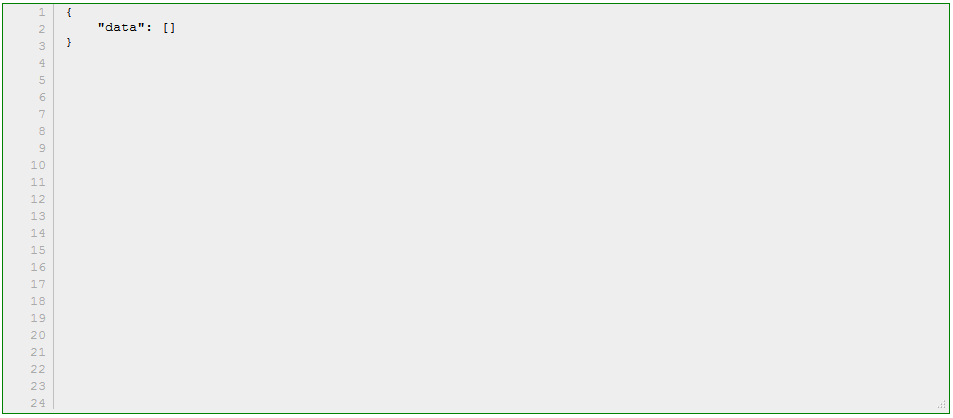
\includegraphics[width=1\textwidth]{images/Anexos/Formato_JSON.png}
		\caption[Formato inicial de los archivos JSON. ]{Formato inicial de los archivos JSON.}
		\label{Formato_json}
	\end{figure}

\subsection*{Anexo B: CascadingDropDown}\addcontentsline{toc}{subsection}{Anexo B: CascadingDropDown}

CascadingDropDown es una extención de ASP.NET AJAX que se puede conectar a un  DropDownList para obtener la población automática de un conjunto de controles DropDownList. Cada vez que se seleeciona uno de los DropDownList, el CascadingDropDown realiza una llamada a un servicio web, para recuperar la lista de valores para poblar el siguiente DropDownList.
\\

\textbf{Propiedades:}
\begin{itemize}


	\item TargetControlID: El ID de la lista desplegable a la que se aplicará.
	
	\item  Category: se define como el nombre de la categoría que la lista desplegable representa. Su utilidad será la de representar uno de los dos parámetros de entrada al ServiceMethod que estudiaremos posteriormente.
	
	\item  PromptText: Es un texto opcional que verá el usuario cuando la lista desplegable esté vacía.
	
	\item  LoadingText: Es un texto opcional que verá el usuario cuando el dato se está cargando.
	
	\item  ServicePath: Es el path del servicio web que devuelve la información que se usará para rellenar la lista desplegable.
	
	\item  ServiceMethod: Es el nombre del método el cual pobla la lista desplegable.
	
	\item  ParentControlID: ID de la lista desplegable de cuya selección depende esta lista desplegable.
	
	\item  SelectedValue: valor que vendría seleccionado por defecto. Es opcional. 
\end{itemize}



La función a la que se llamará  para rellenar la lista desplegable tendrá el siguiente formato:

 \lstset{language=C, breaklines=true, basicstyle=\footnotesize}
 \begin{lstlisting}[frame=single]
[WebMethod]

public CascadingDropDownNameValue[] GetDropDownContents(string knownCategoryValues, string category){

...
} 
 \end{lstlisting}
 
 Se puede observar que:
 \begin{itemize}
 	\item La función debe ir precedida por [WebMethod].
 	\item CascadingDropDownNameValue es un tipo de dato dentro del namespace AjaxControlToolkit.
 	\item El segundo parámetro (category)  corresponde al atributo Category que  se ha definido previamente en el control CascadingDropDown. 
 \end{itemize}



\end{document} 